\batchmode
\documentclass[a4paper]{book}
\usepackage{makeidx}
\usepackage{natbib}
\usepackage{graphicx}
\usepackage{multicol}
\usepackage{float}
\usepackage{listings}
\usepackage{color}
\usepackage{ifthen}
\usepackage[table]{xcolor}
\usepackage{textcomp}
\usepackage{alltt}
\usepackage[utf8]{inputenc}
\usepackage{mathptmx}
\usepackage[scaled=.90]{helvet}
\usepackage{courier}
\usepackage{sectsty}
\usepackage[titles]{tocloft}
\usepackage{doxygen}
\lstset{language=C++,inputencoding=utf8,basicstyle=\footnotesize,breaklines=true,breakatwhitespace=true,tabsize=8,numbers=left }
\makeindex
\setcounter{tocdepth}{3}
\renewcommand{\footrulewidth}{0.4pt}
\renewcommand{\familydefault}{\sfdefault}
\hfuzz=15pt
\setlength{\emergencystretch}{15pt}
\hbadness=750
\tolerance=750
\begin{document}
\begin{titlepage}
\vspace*{7cm}
\begin{center}
{\Large dcsl\-\_\-messages }\\
\vspace*{1cm}
{\large \-Generated by Doxygen 1.7.6.1}\\
\vspace*{0.5cm}
{\small Fri Jan 18 2013 20:40:14}\\
\end{center}
\end{titlepage}
\clearemptydoublepage
\pagenumbering{roman}
\tableofcontents
\clearemptydoublepage
\pagenumbering{arabic}
\chapter{\-Main \-Page}
\label{index}

{\bfseries dcsl\-\_\-high\-\_\-level\-\_\-control} 

\-This package provides \char`\"{}high level control\char`\"{} for planar robots. \-The dcsl\-\_\-miabot\-\_\-follower\-\_\-control node implements an algorithm to cause robots to follow or 'chase' one another. \-The \-C++ library dcsl\-\_\-miabot\-\_\-high\-\_\-level\-\_\-math provides the control law for that node.

\-Launchfiles are also included to create ipc-\/bridge nodes that allow control algorithms written in \-Matlab to be called from \-R\-O\-S. \-Sample \-Matlab node and control law files are included within the matlab folder. \-Issues with installation of ipc-\/bridge have kept us from testing that functionality.\section{\-R\-O\-S A\-P\-I}\label{index_rosapi}
\-List of nodes\-:
\begin{DoxyItemize}
\item {\bfseries \doxyref{dcsl\-\_\-miabot\-\_\-follower\-\_\-control.\-cc}{p.}{dcsl__miabot__follower__control_8cc}} 
\end{DoxyItemize}

\-List of libraries\-:
\begin{DoxyItemize}
\item {\bfseries \doxyref{dcsl\-\_\-miabot\-\_\-high\-\_\-level\-\_\-math.\-h}{p.}{dcsl__miabot__high__level__math_8h}} 
\end{DoxyItemize}

\-List of launchfiles
\begin{DoxyItemize}
\item {\bfseries miabot\-\_\-high\-\_\-level} 
\item {\bfseries test\-\_\-pose\-\_\-array\-\_\-subsciber} 
\end{DoxyItemize}



\subsection{dcsl\-\_\-miabot\-\_\-follower\-\_\-control}\label{index_dcsl_high_level_control}
\-This node subscribes to robot state estimates in \-Pose\-Array form, and calculates and publishes waypoints in \-Pose\-Array form such that the robots will follow each other.\subsection{\-Usage}\label{index_usage}
\begin{DoxyVerb}
$ dcsl_miabot_follower_control [standard ROS args]
\end{DoxyVerb}
\subsubsection{\-R\-O\-S topics}\label{index_topics}
\-Subscribes to (name / type)\-:
\begin{DoxyItemize}
\item {\bfseries \char`\"{}state\-\_\-estimate/\-Pose\-Array\char`\"{}} \-: array \char`\"{}poses\char`\"{} holds estimate of current pose for each robot.
\end{DoxyItemize}

\-Publishes to (name / type)\-:
\begin{DoxyItemize}
\item {\bfseries \char`\"{}waypoint\-\_\-input/\-Pose\-Array\char`\"{}} \-: array \char`\"{}poses\char`\"{} holds desired pose waypoint for each robot.
\end{DoxyItemize}\subsubsection{\-R\-O\-S parameters}\label{index_parameters}

\begin{DoxyItemize}
\item {\bfseries \char`\"{}/n\-\_\-robots\char`\"{}} \-: \-Number of robots to be controlled.
\end{DoxyItemize}



\subsection{dcsl\-\_\-miabot\-\_\-high\-\_\-level\-\_\-math}\label{index_dcsl_miabot_high_level_math}
\-This is a \-C++ shared-\/object library that includes the math functions used in the dcsl\-\_\-miabot\-\_\-high\-\_\-level\-\_\-control package. 
\chapter{\-Namespace \-Index}
\section{\-Namespace \-List}
\-Here is a list of all namespaces with brief descriptions\-:\begin{DoxyCompactList}
\item\contentsline{section}{{\bf dcsl\-\_\-swarm\-\_\-director\-\_\-node} }{\pageref{namespacedcsl__swarm__director__node}}{}
\end{DoxyCompactList}

\chapter{\-Class \-Index}
\section{\-Class \-List}
\-Here are the classes, structs, unions and interfaces with brief descriptions\-:\begin{DoxyCompactList}
\item\contentsline{section}{{\bf \-Miabot\-Follower\-Controller} \\*\doxyref{\-Miabot\-Follower\-Controller}{p.}{classMiabotFollowerController} class handles callbacks for miabot\-\_\-follower\-\_\-control node }{\pageref{classMiabotFollowerController}}{}
\end{DoxyCompactList}

\chapter{\-File \-Index}
\section{\-File \-List}
\-Here is a list of all files with brief descriptions\-:\begin{DoxyCompactList}
\item\contentsline{section}{{\bf \-\_\-\-\_\-init\-\_\-\-\_\-.\-py} }{\pageref{____init_____8py}}{}
\item\contentsline{section}{{\bf msg/\-\_\-\-\_\-init\-\_\-\-\_\-.\-py} }{\pageref{msg_2____init_____8py}}{}
\item\contentsline{section}{{\bf \-\_\-beluga\-Input.\-py} }{\pageref{__belugaInput_8py}}{}
\item\contentsline{section}{{\bf \-\_\-\-Twist\-Array.\-py} }{\pageref{__TwistArray_8py}}{}
\item\contentsline{section}{{\bf beluga\-Input.\-h} }{\pageref{belugaInput_8h}}{}
\item\contentsline{section}{{\bf \-Twist\-Array.\-h} }{\pageref{TwistArray_8h}}{}
\end{DoxyCompactList}

\chapter{\-Namespace \-Documentation}
\section{dcsl\-\_\-messages \-Namespace \-Reference}
\label{namespacedcsl__messages}\index{dcsl\-\_\-messages@{dcsl\-\_\-messages}}
\subsection*{\-Namespaces}
\begin{DoxyCompactItemize}
\item 
namespace {\bf msg}
\end{DoxyCompactItemize}
\subsection*{\-Classes}
\begin{DoxyCompactItemize}
\item 
struct {\bf beluga\-Input\-\_\-}
\item 
struct {\bf \-Twist\-Array\-\_\-}
\end{DoxyCompactItemize}
\subsection*{\-Typedefs}
\begin{DoxyCompactItemize}
\item 
typedef \*
\-::{\bf dcsl\-\_\-messages\-::beluga\-Input\-\_\-}\*
$<$ std\-::allocator$<$ void $>$ $>$ {\bf beluga\-Input}
\item 
typedef boost\-::shared\-\_\-ptr\*
$<$ \-::{\bf dcsl\-\_\-messages\-::beluga\-Input} \*
const  $>$ {\bf beluga\-Input\-Const\-Ptr}
\item 
typedef boost\-::shared\-\_\-ptr\*
$<$ \-::{\bf dcsl\-\_\-messages\-::beluga\-Input} $>$ {\bf beluga\-Input\-Ptr}
\item 
typedef \*
\-::{\bf dcsl\-\_\-messages\-::\-Twist\-Array\-\_\-}\*
$<$ std\-::allocator$<$ void $>$ $>$ {\bf \-Twist\-Array}
\item 
typedef boost\-::shared\-\_\-ptr\*
$<$ \-::{\bf dcsl\-\_\-messages\-::\-Twist\-Array} \*
const  $>$ {\bf \-Twist\-Array\-Const\-Ptr}
\item 
typedef boost\-::shared\-\_\-ptr\*
$<$ \-::{\bf dcsl\-\_\-messages\-::\-Twist\-Array} $>$ {\bf \-Twist\-Array\-Ptr}
\end{DoxyCompactItemize}
\subsection*{\-Functions}
\begin{DoxyCompactItemize}
\item 
{\footnotesize template$<$typename Container\-Allocator $>$ }\\std\-::ostream \& {\bf operator$<$$<$} (std\-::ostream \&s, const \-::{\bf dcsl\-\_\-messages\-::\-Twist\-Array\-\_\-}$<$ \-Container\-Allocator $>$ \&v)
\item 
{\footnotesize template$<$typename Container\-Allocator $>$ }\\std\-::ostream \& {\bf operator$<$$<$} (std\-::ostream \&s, const \-::{\bf dcsl\-\_\-messages\-::beluga\-Input\-\_\-}$<$ \-Container\-Allocator $>$ \&v)
\end{DoxyCompactItemize}


\subsection{\-Typedef \-Documentation}
\index{dcsl\-\_\-messages@{dcsl\-\_\-messages}!beluga\-Input@{beluga\-Input}}
\index{beluga\-Input@{beluga\-Input}!dcsl_messages@{dcsl\-\_\-messages}}
\subsubsection[{beluga\-Input}]{\setlength{\rightskip}{0pt plus 5cm}typedef \-::{\bf dcsl\-\_\-messages\-::beluga\-Input\-\_\-}$<$std\-::allocator$<$void$>$ $>$ {\bf dcsl\-\_\-messages\-::beluga\-Input}}\label{namespacedcsl__messages_aaa07218fd9bb3b31cb9d855e68a1bf03}


\-Definition at line 52 of file beluga\-Input.\-h.

\index{dcsl\-\_\-messages@{dcsl\-\_\-messages}!beluga\-Input\-Const\-Ptr@{beluga\-Input\-Const\-Ptr}}
\index{beluga\-Input\-Const\-Ptr@{beluga\-Input\-Const\-Ptr}!dcsl_messages@{dcsl\-\_\-messages}}
\subsubsection[{beluga\-Input\-Const\-Ptr}]{\setlength{\rightskip}{0pt plus 5cm}typedef boost\-::shared\-\_\-ptr$<$ \-::{\bf dcsl\-\_\-messages\-::beluga\-Input} const$>$ {\bf dcsl\-\_\-messages\-::beluga\-Input\-Const\-Ptr}}\label{namespacedcsl__messages_ad097cf5a7e8480b9ea2bb393b27a7ded}


\-Definition at line 55 of file beluga\-Input.\-h.

\index{dcsl\-\_\-messages@{dcsl\-\_\-messages}!beluga\-Input\-Ptr@{beluga\-Input\-Ptr}}
\index{beluga\-Input\-Ptr@{beluga\-Input\-Ptr}!dcsl_messages@{dcsl\-\_\-messages}}
\subsubsection[{beluga\-Input\-Ptr}]{\setlength{\rightskip}{0pt plus 5cm}typedef boost\-::shared\-\_\-ptr$<$ \-::{\bf dcsl\-\_\-messages\-::beluga\-Input}$>$ {\bf dcsl\-\_\-messages\-::beluga\-Input\-Ptr}}\label{namespacedcsl__messages_a496d32e6f48704627157a768aff69eaa}


\-Definition at line 54 of file beluga\-Input.\-h.

\index{dcsl\-\_\-messages@{dcsl\-\_\-messages}!\-Twist\-Array@{\-Twist\-Array}}
\index{\-Twist\-Array@{\-Twist\-Array}!dcsl_messages@{dcsl\-\_\-messages}}
\subsubsection[{\-Twist\-Array}]{\setlength{\rightskip}{0pt plus 5cm}typedef \-::{\bf dcsl\-\_\-messages\-::\-Twist\-Array\-\_\-}$<$std\-::allocator$<$void$>$ $>$ {\bf dcsl\-\_\-messages\-::\-Twist\-Array}}\label{namespacedcsl__messages_ae080f2840b4047dfc36e5e2d9ddea6dd}


\-Definition at line 49 of file \-Twist\-Array.\-h.

\index{dcsl\-\_\-messages@{dcsl\-\_\-messages}!\-Twist\-Array\-Const\-Ptr@{\-Twist\-Array\-Const\-Ptr}}
\index{\-Twist\-Array\-Const\-Ptr@{\-Twist\-Array\-Const\-Ptr}!dcsl_messages@{dcsl\-\_\-messages}}
\subsubsection[{\-Twist\-Array\-Const\-Ptr}]{\setlength{\rightskip}{0pt plus 5cm}typedef boost\-::shared\-\_\-ptr$<$ \-::{\bf dcsl\-\_\-messages\-::\-Twist\-Array} const$>$ {\bf dcsl\-\_\-messages\-::\-Twist\-Array\-Const\-Ptr}}\label{namespacedcsl__messages_ad97b1d7c5d2837b4bf75c2ad2dddf357}


\-Definition at line 52 of file \-Twist\-Array.\-h.

\index{dcsl\-\_\-messages@{dcsl\-\_\-messages}!\-Twist\-Array\-Ptr@{\-Twist\-Array\-Ptr}}
\index{\-Twist\-Array\-Ptr@{\-Twist\-Array\-Ptr}!dcsl_messages@{dcsl\-\_\-messages}}
\subsubsection[{\-Twist\-Array\-Ptr}]{\setlength{\rightskip}{0pt plus 5cm}typedef boost\-::shared\-\_\-ptr$<$ \-::{\bf dcsl\-\_\-messages\-::\-Twist\-Array}$>$ {\bf dcsl\-\_\-messages\-::\-Twist\-Array\-Ptr}}\label{namespacedcsl__messages_a89b2c91c66ea4850948805eced98bdd3}


\-Definition at line 51 of file \-Twist\-Array.\-h.



\subsection{\-Function \-Documentation}
\index{dcsl\-\_\-messages@{dcsl\-\_\-messages}!operator$<$$<$@{operator$<$$<$}}
\index{operator$<$$<$@{operator$<$$<$}!dcsl_messages@{dcsl\-\_\-messages}}
\subsubsection[{operator$<$$<$}]{\setlength{\rightskip}{0pt plus 5cm}template$<$typename Container\-Allocator $>$ std\-::ostream\& dcsl\-\_\-messages\-::operator$<$$<$ (
\begin{DoxyParamCaption}
\item[{std\-::ostream \&}]{s, }
\item[{const \-::{\bf dcsl\-\_\-messages\-::\-Twist\-Array\-\_\-}$<$ \-Container\-Allocator $>$ \&}]{v}
\end{DoxyParamCaption}
)}\label{namespacedcsl__messages_ad04676e57117bfab15f782950e90fb45}


\-Definition at line 56 of file \-Twist\-Array.\-h.

\index{dcsl\-\_\-messages@{dcsl\-\_\-messages}!operator$<$$<$@{operator$<$$<$}}
\index{operator$<$$<$@{operator$<$$<$}!dcsl_messages@{dcsl\-\_\-messages}}
\subsubsection[{operator$<$$<$}]{\setlength{\rightskip}{0pt plus 5cm}template$<$typename Container\-Allocator $>$ std\-::ostream\& dcsl\-\_\-messages\-::operator$<$$<$ (
\begin{DoxyParamCaption}
\item[{std\-::ostream \&}]{s, }
\item[{const \-::{\bf dcsl\-\_\-messages\-::beluga\-Input\-\_\-}$<$ \-Container\-Allocator $>$ \&}]{v}
\end{DoxyParamCaption}
)}\label{namespacedcsl__messages_aefdd5edcac8a39797ab06057f9e40d9e}


\-Definition at line 59 of file beluga\-Input.\-h.


\section{dcsl\-\_\-messages\-:\-:msg \-Namespace \-Reference}
\label{namespacedcsl__messages_1_1msg}\index{dcsl\-\_\-messages\-::msg@{dcsl\-\_\-messages\-::msg}}
\subsection*{\-Namespaces}
\begin{DoxyCompactItemize}
\item 
namespace {\bf \-\_\-beluga\-Input}
\item 
namespace {\bf \-\_\-\-Twist\-Array}
\end{DoxyCompactItemize}

\section{dcsl\-\_\-messages\-:\-:msg\-:\-:\-\_\-beluga\-Input \-Namespace \-Reference}
\label{namespacedcsl__messages_1_1msg_1_1__belugaInput}\index{dcsl\-\_\-messages\-::msg\-::\-\_\-beluga\-Input@{dcsl\-\_\-messages\-::msg\-::\-\_\-beluga\-Input}}
\subsection*{\-Classes}
\begin{DoxyCompactItemize}
\item 
class {\bf beluga\-Input}
\end{DoxyCompactItemize}
\subsection*{\-Variables}
\begin{DoxyCompactItemize}
\item 
tuple {\bf \-\_\-struct\-\_\-3h} = struct.\-Struct(\char`\"{}$<$3h\char`\"{})
\item 
{\bf \-\_\-struct\-\_\-\-I} = genpy.\-struct\-\_\-\-I
\item 
int {\bf python3} = 0x03000000
\end{DoxyCompactItemize}


\subsection{\-Detailed \-Description}
\begin{DoxyVerb}autogenerated by genpy from dcsl_messages/belugaInput.msg. Do not edit.\end{DoxyVerb}
 

\subsection{\-Variable \-Documentation}
\index{dcsl\-\_\-messages\-::msg\-::\-\_\-beluga\-Input@{dcsl\-\_\-messages\-::msg\-::\-\_\-beluga\-Input}!\-\_\-struct\-\_\-3h@{\-\_\-struct\-\_\-3h}}
\index{\-\_\-struct\-\_\-3h@{\-\_\-struct\-\_\-3h}!dcsl_messages::msg::_belugaInput@{dcsl\-\_\-messages\-::msg\-::\-\_\-beluga\-Input}}
\subsubsection[{\-\_\-struct\-\_\-3h}]{\setlength{\rightskip}{0pt plus 5cm}tuple {\bf dcsl\-\_\-messages\-::msg\-::\-\_\-beluga\-Input\-::\-\_\-struct\-\_\-3h} = struct.\-Struct(\char`\"{}$<$3h\char`\"{})}\label{namespacedcsl__messages_1_1msg_1_1__belugaInput_a608573c0c8e4d16587d0e322fbcc126b}


\-Definition at line 113 of file \-\_\-beluga\-Input.\-py.

\index{dcsl\-\_\-messages\-::msg\-::\-\_\-beluga\-Input@{dcsl\-\_\-messages\-::msg\-::\-\_\-beluga\-Input}!\-\_\-struct\-\_\-\-I@{\-\_\-struct\-\_\-\-I}}
\index{\-\_\-struct\-\_\-\-I@{\-\_\-struct\-\_\-\-I}!dcsl_messages::msg::_belugaInput@{dcsl\-\_\-messages\-::msg\-::\-\_\-beluga\-Input}}
\subsubsection[{\-\_\-struct\-\_\-\-I}]{\setlength{\rightskip}{0pt plus 5cm}{\bf dcsl\-\_\-messages\-::msg\-::\-\_\-beluga\-Input\-::\-\_\-struct\-\_\-\-I} = genpy.\-struct\-\_\-\-I}\label{namespacedcsl__messages_1_1msg_1_1__belugaInput_a4cde2c535e2b71a38fec4d5b6faff4d8}


\-Definition at line 112 of file \-\_\-beluga\-Input.\-py.

\index{dcsl\-\_\-messages\-::msg\-::\-\_\-beluga\-Input@{dcsl\-\_\-messages\-::msg\-::\-\_\-beluga\-Input}!python3@{python3}}
\index{python3@{python3}!dcsl_messages::msg::_belugaInput@{dcsl\-\_\-messages\-::msg\-::\-\_\-beluga\-Input}}
\subsubsection[{python3}]{\setlength{\rightskip}{0pt plus 5cm}int {\bf dcsl\-\_\-messages\-::msg\-::\-\_\-beluga\-Input\-::python3} = 0x03000000}\label{namespacedcsl__messages_1_1msg_1_1__belugaInput_a4d8691db4eb6ea8d9a2d2dd150f8ae44}


\-Definition at line 3 of file \-\_\-beluga\-Input.\-py.


\section{dcsl\-\_\-messages\-:\-:msg\-:\-:\-\_\-\-Twist\-Array \-Namespace \-Reference}
\label{namespacedcsl__messages_1_1msg_1_1__TwistArray}\index{dcsl\-\_\-messages\-::msg\-::\-\_\-\-Twist\-Array@{dcsl\-\_\-messages\-::msg\-::\-\_\-\-Twist\-Array}}
\subsection*{\-Classes}
\begin{DoxyCompactItemize}
\item 
class {\bf \-Twist\-Array}
\end{DoxyCompactItemize}
\subsection*{\-Variables}
\begin{DoxyCompactItemize}
\item 
tuple {\bf \-\_\-struct\-\_\-3d} = struct.\-Struct(\char`\"{}$<$3d\char`\"{})
\item 
tuple {\bf \-\_\-struct\-\_\-3\-I} = struct.\-Struct(\char`\"{}$<$3\-I\char`\"{})
\item 
{\bf \-\_\-struct\-\_\-\-I} = genpy.\-struct\-\_\-\-I
\item 
int {\bf python3} = 0x03000000
\end{DoxyCompactItemize}


\subsection{\-Detailed \-Description}
\begin{DoxyVerb}autogenerated by genpy from dcsl_messages/TwistArray.msg. Do not edit.\end{DoxyVerb}
 

\subsection{\-Variable \-Documentation}
\index{dcsl\-\_\-messages\-::msg\-::\-\_\-\-Twist\-Array@{dcsl\-\_\-messages\-::msg\-::\-\_\-\-Twist\-Array}!\-\_\-struct\-\_\-3d@{\-\_\-struct\-\_\-3d}}
\index{\-\_\-struct\-\_\-3d@{\-\_\-struct\-\_\-3d}!dcsl_messages::msg::_TwistArray@{dcsl\-\_\-messages\-::msg\-::\-\_\-\-Twist\-Array}}
\subsubsection[{\-\_\-struct\-\_\-3d}]{\setlength{\rightskip}{0pt plus 5cm}tuple {\bf dcsl\-\_\-messages\-::msg\-::\-\_\-\-Twist\-Array\-::\-\_\-struct\-\_\-3d} = struct.\-Struct(\char`\"{}$<$3d\char`\"{})}\label{namespacedcsl__messages_1_1msg_1_1__TwistArray_a80971b2cf8cb24c8f4f464c040c1a380}


\-Definition at line 233 of file \-\_\-\-Twist\-Array.\-py.

\index{dcsl\-\_\-messages\-::msg\-::\-\_\-\-Twist\-Array@{dcsl\-\_\-messages\-::msg\-::\-\_\-\-Twist\-Array}!\-\_\-struct\-\_\-3\-I@{\-\_\-struct\-\_\-3\-I}}
\index{\-\_\-struct\-\_\-3\-I@{\-\_\-struct\-\_\-3\-I}!dcsl_messages::msg::_TwistArray@{dcsl\-\_\-messages\-::msg\-::\-\_\-\-Twist\-Array}}
\subsubsection[{\-\_\-struct\-\_\-3\-I}]{\setlength{\rightskip}{0pt plus 5cm}tuple {\bf dcsl\-\_\-messages\-::msg\-::\-\_\-\-Twist\-Array\-::\-\_\-struct\-\_\-3\-I} = struct.\-Struct(\char`\"{}$<$3\-I\char`\"{})}\label{namespacedcsl__messages_1_1msg_1_1__TwistArray_a2f16a2dfc4a4dc778f479718aaf41382}


\-Definition at line 232 of file \-\_\-\-Twist\-Array.\-py.

\index{dcsl\-\_\-messages\-::msg\-::\-\_\-\-Twist\-Array@{dcsl\-\_\-messages\-::msg\-::\-\_\-\-Twist\-Array}!\-\_\-struct\-\_\-\-I@{\-\_\-struct\-\_\-\-I}}
\index{\-\_\-struct\-\_\-\-I@{\-\_\-struct\-\_\-\-I}!dcsl_messages::msg::_TwistArray@{dcsl\-\_\-messages\-::msg\-::\-\_\-\-Twist\-Array}}
\subsubsection[{\-\_\-struct\-\_\-\-I}]{\setlength{\rightskip}{0pt plus 5cm}{\bf dcsl\-\_\-messages\-::msg\-::\-\_\-\-Twist\-Array\-::\-\_\-struct\-\_\-\-I} = genpy.\-struct\-\_\-\-I}\label{namespacedcsl__messages_1_1msg_1_1__TwistArray_abf84c0505fc650e34c579fe88152d944}


\-Definition at line 231 of file \-\_\-\-Twist\-Array.\-py.

\index{dcsl\-\_\-messages\-::msg\-::\-\_\-\-Twist\-Array@{dcsl\-\_\-messages\-::msg\-::\-\_\-\-Twist\-Array}!python3@{python3}}
\index{python3@{python3}!dcsl_messages::msg::_TwistArray@{dcsl\-\_\-messages\-::msg\-::\-\_\-\-Twist\-Array}}
\subsubsection[{python3}]{\setlength{\rightskip}{0pt plus 5cm}int {\bf dcsl\-\_\-messages\-::msg\-::\-\_\-\-Twist\-Array\-::python3} = 0x03000000}\label{namespacedcsl__messages_1_1msg_1_1__TwistArray_a8022ba0b388d74060e0700628f1b8073}


\-Definition at line 3 of file \-\_\-\-Twist\-Array.\-py.


\section{ros \-Namespace \-Reference}
\label{namespaceros}\index{ros@{ros}}
\subsection*{\-Namespaces}
\begin{DoxyCompactItemize}
\item 
namespace {\bf message\-\_\-operations}
\item 
namespace {\bf message\-\_\-traits}
\item 
namespace {\bf serialization}
\end{DoxyCompactItemize}

\section{ros\-:\-:message\-\_\-operations \-Namespace \-Reference}
\label{namespaceros_1_1message__operations}\index{ros\-::message\-\_\-operations@{ros\-::message\-\_\-operations}}
\subsection*{\-Classes}
\begin{DoxyCompactItemize}
\item 
struct {\bf \-Printer$<$ \-::dcsl\-\_\-messages\-::beluga\-Input\-\_\-$<$ Container\-Allocator $>$ $>$}
\item 
struct {\bf \-Printer$<$ \-::dcsl\-\_\-messages\-::\-Twist\-Array\-\_\-$<$ Container\-Allocator $>$ $>$}
\end{DoxyCompactItemize}

\section{ros\-:\-:message\-\_\-traits \-Namespace \-Reference}
\label{namespaceros_1_1message__traits}\index{ros\-::message\-\_\-traits@{ros\-::message\-\_\-traits}}
\subsection*{\-Classes}
\begin{DoxyCompactItemize}
\item 
struct {\bf \-Data\-Type$<$ \-::dcsl\-\_\-messages\-::beluga\-Input\-\_\-$<$ Container\-Allocator $>$ $>$}
\item 
struct {\bf \-Data\-Type$<$ \-::dcsl\-\_\-messages\-::\-Twist\-Array\-\_\-$<$ Container\-Allocator $>$ $>$}
\item 
struct {\bf \-Definition$<$ \-::dcsl\-\_\-messages\-::beluga\-Input\-\_\-$<$ Container\-Allocator $>$ $>$}
\item 
struct {\bf \-Definition$<$ \-::dcsl\-\_\-messages\-::\-Twist\-Array\-\_\-$<$ Container\-Allocator $>$ $>$}
\item 
struct {\bf \-Has\-Header$<$ \-::dcsl\-\_\-messages\-::\-Twist\-Array\-\_\-$<$ Container\-Allocator $>$ $>$}
\item 
struct {\bf \-Has\-Header$<$ const \-::dcsl\-\_\-messages\-::\-Twist\-Array\-\_\-$<$ Container\-Allocator $>$ $>$}
\item 
struct {\bf \-Is\-Fixed\-Size$<$ \-::dcsl\-\_\-messages\-::beluga\-Input\-\_\-$<$ Container\-Allocator $>$ $>$}
\item 
struct {\bf \-Is\-Message$<$ \-::dcsl\-\_\-messages\-::beluga\-Input\-\_\-$<$ Container\-Allocator $>$ $>$}
\item 
struct {\bf \-Is\-Message$<$ \-::dcsl\-\_\-messages\-::beluga\-Input\-\_\-$<$ Container\-Allocator $>$const  $>$}
\item 
struct {\bf \-Is\-Message$<$ \-::dcsl\-\_\-messages\-::\-Twist\-Array\-\_\-$<$ Container\-Allocator $>$ $>$}
\item 
struct {\bf \-Is\-Message$<$ \-::dcsl\-\_\-messages\-::\-Twist\-Array\-\_\-$<$ Container\-Allocator $>$const  $>$}
\item 
struct {\bf \-M\-D5\-Sum$<$ \-::dcsl\-\_\-messages\-::beluga\-Input\-\_\-$<$ Container\-Allocator $>$ $>$}
\item 
struct {\bf \-M\-D5\-Sum$<$ \-::dcsl\-\_\-messages\-::\-Twist\-Array\-\_\-$<$ Container\-Allocator $>$ $>$}
\end{DoxyCompactItemize}

\section{ros\-:\-:serialization \-Namespace \-Reference}
\label{namespaceros_1_1serialization}\index{ros\-::serialization@{ros\-::serialization}}
\subsection*{\-Classes}
\begin{DoxyCompactItemize}
\item 
struct {\bf \-Serializer$<$ \-::dcsl\-\_\-messages\-::beluga\-Input\-\_\-$<$ Container\-Allocator $>$ $>$}
\item 
struct {\bf \-Serializer$<$ \-::dcsl\-\_\-messages\-::\-Twist\-Array\-\_\-$<$ Container\-Allocator $>$ $>$}
\end{DoxyCompactItemize}

\chapter{\-Class \-Documentation}
\section{dcsl\-\_\-messages.\-msg.\-\_\-beluga\-Input.\-beluga\-Input \-Class \-Reference}
\label{classdcsl__messages_1_1msg_1_1__belugaInput_1_1belugaInput}\index{dcsl\-\_\-messages.\-msg.\-\_\-beluga\-Input.\-beluga\-Input@{dcsl\-\_\-messages.\-msg.\-\_\-beluga\-Input.\-beluga\-Input}}
\subsection*{\-Public \-Member \-Functions}
\begin{DoxyCompactItemize}
\item 
def {\bf \-\_\-\-\_\-init\-\_\-\-\_\-}
\item 
def {\bf deserialize}
\item 
def {\bf deserialize\-\_\-numpy}
\item 
def {\bf serialize}
\item 
def {\bf serialize\-\_\-numpy}
\end{DoxyCompactItemize}
\subsection*{\-Public \-Attributes}
\begin{DoxyCompactItemize}
\item 
{\bf servo}
\item 
{\bf thrust\-\_\-motor}
\item 
{\bf vertical\-\_\-motor}
\end{DoxyCompactItemize}
\subsection*{\-Private \-Member \-Functions}
\begin{DoxyCompactItemize}
\item 
def {\bf \-\_\-get\-\_\-types}
\end{DoxyCompactItemize}
\subsection*{\-Static \-Private \-Attributes}
\begin{DoxyCompactItemize}
\item 
list {\bf \-\_\-\-\_\-slots\-\_\-\-\_\-} = ['{\bf vertical\-\_\-motor}','{\bf thrust\-\_\-motor}','{\bf servo}']
\item 
string {\bf \-\_\-full\-\_\-text}
\item 
{\bf \-\_\-has\-\_\-header} = \-False
\item 
string {\bf \-\_\-md5sum} = \char`\"{}d7a8a4a3ad3fa031c886b7c16b438163\char`\"{}
\item 
list {\bf \-\_\-slot\-\_\-types} = ['int16','int16','int16']
\item 
string {\bf \-\_\-type} = \char`\"{}dcsl\-\_\-messages/{\bf beluga\-Input}\char`\"{}
\end{DoxyCompactItemize}


\subsection{\-Detailed \-Description}


\-Definition at line 8 of file \-\_\-beluga\-Input.\-py.



\subsection{\-Constructor \& \-Destructor \-Documentation}
\index{dcsl\-\_\-messages\-::msg\-::\-\_\-beluga\-Input\-::beluga\-Input@{dcsl\-\_\-messages\-::msg\-::\-\_\-beluga\-Input\-::beluga\-Input}!\-\_\-\-\_\-init\-\_\-\-\_\-@{\-\_\-\-\_\-init\-\_\-\-\_\-}}
\index{\-\_\-\-\_\-init\-\_\-\-\_\-@{\-\_\-\-\_\-init\-\_\-\-\_\-}!dcsl_messages::msg::_belugaInput::belugaInput@{dcsl\-\_\-messages\-::msg\-::\-\_\-beluga\-Input\-::beluga\-Input}}
\subsubsection[{\-\_\-\-\_\-init\-\_\-\-\_\-}]{\setlength{\rightskip}{0pt plus 5cm}def {\bf dcsl\-\_\-messages.\-msg.\-\_\-beluga\-Input.\-beluga\-Input.\-\_\-\-\_\-init\-\_\-\-\_\-} (
\begin{DoxyParamCaption}
\item[{}]{self, }
\item[{}]{args, }
\item[{}]{kwds}
\end{DoxyParamCaption}
)}\label{classdcsl__messages_1_1msg_1_1__belugaInput_1_1belugaInput_ae81a9e20faf50fc115b34c13ec1e0651}
\begin{DoxyVerb}
Constructor. Any message fields that are implicitly/explicitly
set to None will be assigned a default value. The recommend
use is keyword arguments as this is more robust to future message
changes.  You cannot mix in-order arguments and keyword arguments.

The available fields are:
   vertical_motor,thrust_motor,servo

:param args: complete set of field values, in .msg order
:param kwds: use keyword arguments corresponding to message field names
to set specific fields.
\end{DoxyVerb}
 

\-Definition at line 23 of file \-\_\-beluga\-Input.\-py.



\subsection{\-Member \-Function \-Documentation}
\index{dcsl\-\_\-messages\-::msg\-::\-\_\-beluga\-Input\-::beluga\-Input@{dcsl\-\_\-messages\-::msg\-::\-\_\-beluga\-Input\-::beluga\-Input}!\-\_\-get\-\_\-types@{\-\_\-get\-\_\-types}}
\index{\-\_\-get\-\_\-types@{\-\_\-get\-\_\-types}!dcsl_messages::msg::_belugaInput::belugaInput@{dcsl\-\_\-messages\-::msg\-::\-\_\-beluga\-Input\-::beluga\-Input}}
\subsubsection[{\-\_\-get\-\_\-types}]{\setlength{\rightskip}{0pt plus 5cm}def {\bf dcsl\-\_\-messages.\-msg.\-\_\-beluga\-Input.\-beluga\-Input.\-\_\-get\-\_\-types} (
\begin{DoxyParamCaption}
\item[{}]{self}
\end{DoxyParamCaption}
)\hspace{0.3cm}{\ttfamily  [private]}}\label{classdcsl__messages_1_1msg_1_1__belugaInput_1_1belugaInput_aba50423560222815aacf94fb9b1616ed}
\begin{DoxyVerb}
internal API method
\end{DoxyVerb}
 

\-Definition at line 51 of file \-\_\-beluga\-Input.\-py.

\index{dcsl\-\_\-messages\-::msg\-::\-\_\-beluga\-Input\-::beluga\-Input@{dcsl\-\_\-messages\-::msg\-::\-\_\-beluga\-Input\-::beluga\-Input}!deserialize@{deserialize}}
\index{deserialize@{deserialize}!dcsl_messages::msg::_belugaInput::belugaInput@{dcsl\-\_\-messages\-::msg\-::\-\_\-beluga\-Input\-::beluga\-Input}}
\subsubsection[{deserialize}]{\setlength{\rightskip}{0pt plus 5cm}def {\bf dcsl\-\_\-messages.\-msg.\-\_\-beluga\-Input.\-beluga\-Input.\-deserialize} (
\begin{DoxyParamCaption}
\item[{}]{self, }
\item[{}]{str}
\end{DoxyParamCaption}
)}\label{classdcsl__messages_1_1msg_1_1__belugaInput_1_1belugaInput_a89c81f7317e3431fa370501cd1937ebb}
\begin{DoxyVerb}
unpack serialized message in str into this message instance
:param str: byte array of serialized message, ``str``
\end{DoxyVerb}
 

\-Definition at line 68 of file \-\_\-beluga\-Input.\-py.

\index{dcsl\-\_\-messages\-::msg\-::\-\_\-beluga\-Input\-::beluga\-Input@{dcsl\-\_\-messages\-::msg\-::\-\_\-beluga\-Input\-::beluga\-Input}!deserialize\-\_\-numpy@{deserialize\-\_\-numpy}}
\index{deserialize\-\_\-numpy@{deserialize\-\_\-numpy}!dcsl_messages::msg::_belugaInput::belugaInput@{dcsl\-\_\-messages\-::msg\-::\-\_\-beluga\-Input\-::beluga\-Input}}
\subsubsection[{deserialize\-\_\-numpy}]{\setlength{\rightskip}{0pt plus 5cm}def {\bf dcsl\-\_\-messages.\-msg.\-\_\-beluga\-Input.\-beluga\-Input.\-deserialize\-\_\-numpy} (
\begin{DoxyParamCaption}
\item[{}]{self, }
\item[{}]{str, }
\item[{}]{numpy}
\end{DoxyParamCaption}
)}\label{classdcsl__messages_1_1msg_1_1__belugaInput_1_1belugaInput_a0d9a2c33515306ff1e5dc4b7bbe9307a}
\begin{DoxyVerb}
unpack serialized message in str into this message instance using numpy for array types
:param str: byte array of serialized message, ``str``
:param numpy: numpy python module
\end{DoxyVerb}
 

\-Definition at line 96 of file \-\_\-beluga\-Input.\-py.

\index{dcsl\-\_\-messages\-::msg\-::\-\_\-beluga\-Input\-::beluga\-Input@{dcsl\-\_\-messages\-::msg\-::\-\_\-beluga\-Input\-::beluga\-Input}!serialize@{serialize}}
\index{serialize@{serialize}!dcsl_messages::msg::_belugaInput::belugaInput@{dcsl\-\_\-messages\-::msg\-::\-\_\-beluga\-Input\-::beluga\-Input}}
\subsubsection[{serialize}]{\setlength{\rightskip}{0pt plus 5cm}def {\bf dcsl\-\_\-messages.\-msg.\-\_\-beluga\-Input.\-beluga\-Input.\-serialize} (
\begin{DoxyParamCaption}
\item[{}]{self, }
\item[{}]{buff}
\end{DoxyParamCaption}
)}\label{classdcsl__messages_1_1msg_1_1__belugaInput_1_1belugaInput_a4f4df3835dfefd771119b54d28d98d13}
\begin{DoxyVerb}
serialize message into buffer
:param buff: buffer, ``StringIO``
\end{DoxyVerb}
 

\-Definition at line 57 of file \-\_\-beluga\-Input.\-py.

\index{dcsl\-\_\-messages\-::msg\-::\-\_\-beluga\-Input\-::beluga\-Input@{dcsl\-\_\-messages\-::msg\-::\-\_\-beluga\-Input\-::beluga\-Input}!serialize\-\_\-numpy@{serialize\-\_\-numpy}}
\index{serialize\-\_\-numpy@{serialize\-\_\-numpy}!dcsl_messages::msg::_belugaInput::belugaInput@{dcsl\-\_\-messages\-::msg\-::\-\_\-beluga\-Input\-::beluga\-Input}}
\subsubsection[{serialize\-\_\-numpy}]{\setlength{\rightskip}{0pt plus 5cm}def {\bf dcsl\-\_\-messages.\-msg.\-\_\-beluga\-Input.\-beluga\-Input.\-serialize\-\_\-numpy} (
\begin{DoxyParamCaption}
\item[{}]{self, }
\item[{}]{buff, }
\item[{}]{numpy}
\end{DoxyParamCaption}
)}\label{classdcsl__messages_1_1msg_1_1__belugaInput_1_1belugaInput_af3c87d6e4b7ae0e5a477b5da98a1575f}
\begin{DoxyVerb}
serialize message with numpy array types into buffer
:param buff: buffer, ``StringIO``
:param numpy: numpy python module
\end{DoxyVerb}
 

\-Definition at line 84 of file \-\_\-beluga\-Input.\-py.



\subsection{\-Member \-Data \-Documentation}
\index{dcsl\-\_\-messages\-::msg\-::\-\_\-beluga\-Input\-::beluga\-Input@{dcsl\-\_\-messages\-::msg\-::\-\_\-beluga\-Input\-::beluga\-Input}!\-\_\-\-\_\-slots\-\_\-\-\_\-@{\-\_\-\-\_\-slots\-\_\-\-\_\-}}
\index{\-\_\-\-\_\-slots\-\_\-\-\_\-@{\-\_\-\-\_\-slots\-\_\-\-\_\-}!dcsl_messages::msg::_belugaInput::belugaInput@{dcsl\-\_\-messages\-::msg\-::\-\_\-beluga\-Input\-::beluga\-Input}}
\subsubsection[{\-\_\-\-\_\-slots\-\_\-\-\_\-}]{\setlength{\rightskip}{0pt plus 5cm}list {\bf dcsl\-\_\-messages\-::msg\-::\-\_\-beluga\-Input.\-beluga\-Input\-::\-\_\-\-\_\-slots\-\_\-\-\_\-} = ['{\bf vertical\-\_\-motor}','{\bf thrust\-\_\-motor}','{\bf servo}']\hspace{0.3cm}{\ttfamily  [static, private]}}\label{classdcsl__messages_1_1msg_1_1__belugaInput_1_1belugaInput_a3a1cced77b7b9dd195ac3b86f322402a}


\-Definition at line 20 of file \-\_\-beluga\-Input.\-py.

\index{dcsl\-\_\-messages\-::msg\-::\-\_\-beluga\-Input\-::beluga\-Input@{dcsl\-\_\-messages\-::msg\-::\-\_\-beluga\-Input\-::beluga\-Input}!\-\_\-full\-\_\-text@{\-\_\-full\-\_\-text}}
\index{\-\_\-full\-\_\-text@{\-\_\-full\-\_\-text}!dcsl_messages::msg::_belugaInput::belugaInput@{dcsl\-\_\-messages\-::msg\-::\-\_\-beluga\-Input\-::beluga\-Input}}
\subsubsection[{\-\_\-full\-\_\-text}]{\setlength{\rightskip}{0pt plus 5cm}string {\bf dcsl\-\_\-messages\-::msg\-::\-\_\-beluga\-Input.\-beluga\-Input\-::\-\_\-full\-\_\-text}\hspace{0.3cm}{\ttfamily  [static, private]}}\label{classdcsl__messages_1_1msg_1_1__belugaInput_1_1belugaInput_a117673671010bbc2ae55814dd97d320f}
{\bfseries \-Initial value\-:}
\begin{DoxyCode}
"""#Actuator inputs for DCSL Beluga Robot
#Motor inputs are -255 to 255, positive values drive up and forwards
       respectively
int16 vertical_motor
int16 thrust_motor
#Servo inputs are -90 TO 90, postive values rotate motor X when viewed from
       above
int16 servo

"""
\end{DoxyCode}


\-Definition at line 12 of file \-\_\-beluga\-Input.\-py.

\index{dcsl\-\_\-messages\-::msg\-::\-\_\-beluga\-Input\-::beluga\-Input@{dcsl\-\_\-messages\-::msg\-::\-\_\-beluga\-Input\-::beluga\-Input}!\-\_\-has\-\_\-header@{\-\_\-has\-\_\-header}}
\index{\-\_\-has\-\_\-header@{\-\_\-has\-\_\-header}!dcsl_messages::msg::_belugaInput::belugaInput@{dcsl\-\_\-messages\-::msg\-::\-\_\-beluga\-Input\-::beluga\-Input}}
\subsubsection[{\-\_\-has\-\_\-header}]{\setlength{\rightskip}{0pt plus 5cm}{\bf dcsl\-\_\-messages\-::msg\-::\-\_\-beluga\-Input.\-beluga\-Input\-::\-\_\-has\-\_\-header} = \-False\hspace{0.3cm}{\ttfamily  [static, private]}}\label{classdcsl__messages_1_1msg_1_1__belugaInput_1_1belugaInput_a7e44b846c25248f7f8e1a4d6bd5df379}


\-Definition at line 11 of file \-\_\-beluga\-Input.\-py.

\index{dcsl\-\_\-messages\-::msg\-::\-\_\-beluga\-Input\-::beluga\-Input@{dcsl\-\_\-messages\-::msg\-::\-\_\-beluga\-Input\-::beluga\-Input}!\-\_\-md5sum@{\-\_\-md5sum}}
\index{\-\_\-md5sum@{\-\_\-md5sum}!dcsl_messages::msg::_belugaInput::belugaInput@{dcsl\-\_\-messages\-::msg\-::\-\_\-beluga\-Input\-::beluga\-Input}}
\subsubsection[{\-\_\-md5sum}]{\setlength{\rightskip}{0pt plus 5cm}string {\bf dcsl\-\_\-messages\-::msg\-::\-\_\-beluga\-Input.\-beluga\-Input\-::\-\_\-md5sum} = \char`\"{}d7a8a4a3ad3fa031c886b7c16b438163\char`\"{}\hspace{0.3cm}{\ttfamily  [static, private]}}\label{classdcsl__messages_1_1msg_1_1__belugaInput_1_1belugaInput_afafc4842821b034411382ed05e779aba}


\-Definition at line 9 of file \-\_\-beluga\-Input.\-py.

\index{dcsl\-\_\-messages\-::msg\-::\-\_\-beluga\-Input\-::beluga\-Input@{dcsl\-\_\-messages\-::msg\-::\-\_\-beluga\-Input\-::beluga\-Input}!\-\_\-slot\-\_\-types@{\-\_\-slot\-\_\-types}}
\index{\-\_\-slot\-\_\-types@{\-\_\-slot\-\_\-types}!dcsl_messages::msg::_belugaInput::belugaInput@{dcsl\-\_\-messages\-::msg\-::\-\_\-beluga\-Input\-::beluga\-Input}}
\subsubsection[{\-\_\-slot\-\_\-types}]{\setlength{\rightskip}{0pt plus 5cm}list {\bf dcsl\-\_\-messages\-::msg\-::\-\_\-beluga\-Input.\-beluga\-Input\-::\-\_\-slot\-\_\-types} = ['int16','int16','int16']\hspace{0.3cm}{\ttfamily  [static, private]}}\label{classdcsl__messages_1_1msg_1_1__belugaInput_1_1belugaInput_aa1fa5e34c3dc96f839e08d60a463ad88}


\-Definition at line 21 of file \-\_\-beluga\-Input.\-py.

\index{dcsl\-\_\-messages\-::msg\-::\-\_\-beluga\-Input\-::beluga\-Input@{dcsl\-\_\-messages\-::msg\-::\-\_\-beluga\-Input\-::beluga\-Input}!\-\_\-type@{\-\_\-type}}
\index{\-\_\-type@{\-\_\-type}!dcsl_messages::msg::_belugaInput::belugaInput@{dcsl\-\_\-messages\-::msg\-::\-\_\-beluga\-Input\-::beluga\-Input}}
\subsubsection[{\-\_\-type}]{\setlength{\rightskip}{0pt plus 5cm}string {\bf dcsl\-\_\-messages\-::msg\-::\-\_\-beluga\-Input.\-beluga\-Input\-::\-\_\-type} = \char`\"{}dcsl\-\_\-messages/{\bf beluga\-Input}\char`\"{}\hspace{0.3cm}{\ttfamily  [static, private]}}\label{classdcsl__messages_1_1msg_1_1__belugaInput_1_1belugaInput_a770c3d5faf05c8a3ef12e1fd3c0fbd62}


\-Definition at line 10 of file \-\_\-beluga\-Input.\-py.

\index{dcsl\-\_\-messages\-::msg\-::\-\_\-beluga\-Input\-::beluga\-Input@{dcsl\-\_\-messages\-::msg\-::\-\_\-beluga\-Input\-::beluga\-Input}!servo@{servo}}
\index{servo@{servo}!dcsl_messages::msg::_belugaInput::belugaInput@{dcsl\-\_\-messages\-::msg\-::\-\_\-beluga\-Input\-::beluga\-Input}}
\subsubsection[{servo}]{\setlength{\rightskip}{0pt plus 5cm}{\bf dcsl\-\_\-messages\-::msg\-::\-\_\-beluga\-Input.\-beluga\-Input\-::servo}}\label{classdcsl__messages_1_1msg_1_1__belugaInput_1_1belugaInput_a7cc4a212caa0e95def417058e51c2b5e}


\-Definition at line 35 of file \-\_\-beluga\-Input.\-py.

\index{dcsl\-\_\-messages\-::msg\-::\-\_\-beluga\-Input\-::beluga\-Input@{dcsl\-\_\-messages\-::msg\-::\-\_\-beluga\-Input\-::beluga\-Input}!thrust\-\_\-motor@{thrust\-\_\-motor}}
\index{thrust\-\_\-motor@{thrust\-\_\-motor}!dcsl_messages::msg::_belugaInput::belugaInput@{dcsl\-\_\-messages\-::msg\-::\-\_\-beluga\-Input\-::beluga\-Input}}
\subsubsection[{thrust\-\_\-motor}]{\setlength{\rightskip}{0pt plus 5cm}{\bf dcsl\-\_\-messages\-::msg\-::\-\_\-beluga\-Input.\-beluga\-Input\-::thrust\-\_\-motor}}\label{classdcsl__messages_1_1msg_1_1__belugaInput_1_1belugaInput_ad08f0286ffb8e435900ac97186d191a1}


\-Definition at line 35 of file \-\_\-beluga\-Input.\-py.

\index{dcsl\-\_\-messages\-::msg\-::\-\_\-beluga\-Input\-::beluga\-Input@{dcsl\-\_\-messages\-::msg\-::\-\_\-beluga\-Input\-::beluga\-Input}!vertical\-\_\-motor@{vertical\-\_\-motor}}
\index{vertical\-\_\-motor@{vertical\-\_\-motor}!dcsl_messages::msg::_belugaInput::belugaInput@{dcsl\-\_\-messages\-::msg\-::\-\_\-beluga\-Input\-::beluga\-Input}}
\subsubsection[{vertical\-\_\-motor}]{\setlength{\rightskip}{0pt plus 5cm}{\bf dcsl\-\_\-messages\-::msg\-::\-\_\-beluga\-Input.\-beluga\-Input\-::vertical\-\_\-motor}}\label{classdcsl__messages_1_1msg_1_1__belugaInput_1_1belugaInput_a26757e70f94e0fc8549bf6df62f9f0c2}


\-Definition at line 35 of file \-\_\-beluga\-Input.\-py.



\-The documentation for this class was generated from the following file\-:\begin{DoxyCompactItemize}
\item 
{\bf \-\_\-beluga\-Input.\-py}\end{DoxyCompactItemize}

\section{dcsl\-\_\-messages\-:\-:beluga\-Input\-\_\-$<$ \-Container\-Allocator $>$ \-Struct \-Template \-Reference}
\label{structdcsl__messages_1_1belugaInput__}\index{dcsl\-\_\-messages\-::beluga\-Input\-\_\-$<$ Container\-Allocator $>$@{dcsl\-\_\-messages\-::beluga\-Input\-\_\-$<$ Container\-Allocator $>$}}


{\ttfamily \#include $<$beluga\-Input.\-h$>$}

\subsection*{\-Public \-Types}
\begin{DoxyCompactItemize}
\item 
typedef int16\-\_\-t {\bf \-\_\-servo\-\_\-type}
\item 
typedef int16\-\_\-t {\bf \-\_\-thrust\-\_\-motor\-\_\-type}
\item 
typedef int16\-\_\-t {\bf \-\_\-vertical\-\_\-motor\-\_\-type}
\item 
typedef boost\-::shared\-\_\-ptr\*
$<$ \-::{\bf dcsl\-\_\-messages\-::beluga\-Input\-\_\-}\*
$<$ \-Container\-Allocator $>$ const  $>$ {\bf \-Const\-Ptr}
\item 
typedef boost\-::shared\-\_\-ptr\*
$<$ \-::{\bf dcsl\-\_\-messages\-::beluga\-Input\-\_\-}\*
$<$ \-Container\-Allocator $>$ $>$ {\bf \-Ptr}
\item 
typedef {\bf beluga\-Input\-\_\-}\*
$<$ \-Container\-Allocator $>$ {\bf \-Type}
\end{DoxyCompactItemize}
\subsection*{\-Public \-Member \-Functions}
\begin{DoxyCompactItemize}
\item 
{\bf beluga\-Input\-\_\-} ()
\item 
{\bf beluga\-Input\-\_\-} (const \-Container\-Allocator \&\-\_\-alloc)
\end{DoxyCompactItemize}
\subsection*{\-Public \-Attributes}
\begin{DoxyCompactItemize}
\item 
boost\-::shared\-\_\-ptr$<$ std\-::map\*
$<$ std\-::string, std\-::string $>$ $>$ {\bf \-\_\-\-\_\-connection\-\_\-header}
\item 
int16\-\_\-t {\bf servo}
\item 
int16\-\_\-t {\bf thrust\-\_\-motor}
\item 
int16\-\_\-t {\bf vertical\-\_\-motor}
\end{DoxyCompactItemize}


\subsection{\-Detailed \-Description}
\subsubsection*{template$<$class Container\-Allocator$>$struct dcsl\-\_\-messages\-::beluga\-Input\-\_\-$<$ Container\-Allocator $>$}



\-Definition at line 21 of file beluga\-Input.\-h.



\subsection{\-Member \-Typedef \-Documentation}
\index{dcsl\-\_\-messages\-::beluga\-Input\-\_\-@{dcsl\-\_\-messages\-::beluga\-Input\-\_\-}!\-\_\-servo\-\_\-type@{\-\_\-servo\-\_\-type}}
\index{\-\_\-servo\-\_\-type@{\-\_\-servo\-\_\-type}!dcsl_messages::belugaInput_@{dcsl\-\_\-messages\-::beluga\-Input\-\_\-}}
\subsubsection[{\-\_\-servo\-\_\-type}]{\setlength{\rightskip}{0pt plus 5cm}template$<$class Container\-Allocator $>$ typedef int16\-\_\-t {\bf dcsl\-\_\-messages\-::beluga\-Input\-\_\-}$<$ \-Container\-Allocator $>$\-::{\bf \-\_\-servo\-\_\-type}}\label{structdcsl__messages_1_1belugaInput___a6d7d7b050e17000047e566310236ae9d}


\-Definition at line 44 of file beluga\-Input.\-h.

\index{dcsl\-\_\-messages\-::beluga\-Input\-\_\-@{dcsl\-\_\-messages\-::beluga\-Input\-\_\-}!\-\_\-thrust\-\_\-motor\-\_\-type@{\-\_\-thrust\-\_\-motor\-\_\-type}}
\index{\-\_\-thrust\-\_\-motor\-\_\-type@{\-\_\-thrust\-\_\-motor\-\_\-type}!dcsl_messages::belugaInput_@{dcsl\-\_\-messages\-::beluga\-Input\-\_\-}}
\subsubsection[{\-\_\-thrust\-\_\-motor\-\_\-type}]{\setlength{\rightskip}{0pt plus 5cm}template$<$class Container\-Allocator $>$ typedef int16\-\_\-t {\bf dcsl\-\_\-messages\-::beluga\-Input\-\_\-}$<$ \-Container\-Allocator $>$\-::{\bf \-\_\-thrust\-\_\-motor\-\_\-type}}\label{structdcsl__messages_1_1belugaInput___a65fe2f3273db34d20ea5c278e3201888}


\-Definition at line 41 of file beluga\-Input.\-h.

\index{dcsl\-\_\-messages\-::beluga\-Input\-\_\-@{dcsl\-\_\-messages\-::beluga\-Input\-\_\-}!\-\_\-vertical\-\_\-motor\-\_\-type@{\-\_\-vertical\-\_\-motor\-\_\-type}}
\index{\-\_\-vertical\-\_\-motor\-\_\-type@{\-\_\-vertical\-\_\-motor\-\_\-type}!dcsl_messages::belugaInput_@{dcsl\-\_\-messages\-::beluga\-Input\-\_\-}}
\subsubsection[{\-\_\-vertical\-\_\-motor\-\_\-type}]{\setlength{\rightskip}{0pt plus 5cm}template$<$class Container\-Allocator $>$ typedef int16\-\_\-t {\bf dcsl\-\_\-messages\-::beluga\-Input\-\_\-}$<$ \-Container\-Allocator $>$\-::{\bf \-\_\-vertical\-\_\-motor\-\_\-type}}\label{structdcsl__messages_1_1belugaInput___a1313758c724e262104dc68cd135eb750}


\-Definition at line 38 of file beluga\-Input.\-h.

\index{dcsl\-\_\-messages\-::beluga\-Input\-\_\-@{dcsl\-\_\-messages\-::beluga\-Input\-\_\-}!\-Const\-Ptr@{\-Const\-Ptr}}
\index{\-Const\-Ptr@{\-Const\-Ptr}!dcsl_messages::belugaInput_@{dcsl\-\_\-messages\-::beluga\-Input\-\_\-}}
\subsubsection[{\-Const\-Ptr}]{\setlength{\rightskip}{0pt plus 5cm}template$<$class Container\-Allocator $>$ typedef boost\-::shared\-\_\-ptr$<$ \-::{\bf dcsl\-\_\-messages\-::beluga\-Input\-\_\-}$<$\-Container\-Allocator$>$ const$>$ {\bf dcsl\-\_\-messages\-::beluga\-Input\-\_\-}$<$ \-Container\-Allocator $>$\-::{\bf \-Const\-Ptr}}\label{structdcsl__messages_1_1belugaInput___a3039b9515e227406789730ef24096460}


\-Definition at line 49 of file beluga\-Input.\-h.

\index{dcsl\-\_\-messages\-::beluga\-Input\-\_\-@{dcsl\-\_\-messages\-::beluga\-Input\-\_\-}!\-Ptr@{\-Ptr}}
\index{\-Ptr@{\-Ptr}!dcsl_messages::belugaInput_@{dcsl\-\_\-messages\-::beluga\-Input\-\_\-}}
\subsubsection[{\-Ptr}]{\setlength{\rightskip}{0pt plus 5cm}template$<$class Container\-Allocator $>$ typedef boost\-::shared\-\_\-ptr$<$ \-::{\bf dcsl\-\_\-messages\-::beluga\-Input\-\_\-}$<$\-Container\-Allocator$>$ $>$ {\bf dcsl\-\_\-messages\-::beluga\-Input\-\_\-}$<$ \-Container\-Allocator $>$\-::{\bf \-Ptr}}\label{structdcsl__messages_1_1belugaInput___ad0b5fe3e0abaa151640c53ccc1e3327c}


\-Definition at line 48 of file beluga\-Input.\-h.

\index{dcsl\-\_\-messages\-::beluga\-Input\-\_\-@{dcsl\-\_\-messages\-::beluga\-Input\-\_\-}!\-Type@{\-Type}}
\index{\-Type@{\-Type}!dcsl_messages::belugaInput_@{dcsl\-\_\-messages\-::beluga\-Input\-\_\-}}
\subsubsection[{\-Type}]{\setlength{\rightskip}{0pt plus 5cm}template$<$class Container\-Allocator $>$ typedef {\bf beluga\-Input\-\_\-}$<$\-Container\-Allocator$>$ {\bf dcsl\-\_\-messages\-::beluga\-Input\-\_\-}$<$ \-Container\-Allocator $>$\-::{\bf \-Type}}\label{structdcsl__messages_1_1belugaInput___a830fcf74e68fd47861ce951e08a78cc8}


\-Definition at line 22 of file beluga\-Input.\-h.



\subsection{\-Constructor \& \-Destructor \-Documentation}
\index{dcsl\-\_\-messages\-::beluga\-Input\-\_\-@{dcsl\-\_\-messages\-::beluga\-Input\-\_\-}!beluga\-Input\-\_\-@{beluga\-Input\-\_\-}}
\index{beluga\-Input\-\_\-@{beluga\-Input\-\_\-}!dcsl_messages::belugaInput_@{dcsl\-\_\-messages\-::beluga\-Input\-\_\-}}
\subsubsection[{beluga\-Input\-\_\-}]{\setlength{\rightskip}{0pt plus 5cm}template$<$class Container\-Allocator $>$ {\bf dcsl\-\_\-messages\-::beluga\-Input\-\_\-}$<$ \-Container\-Allocator $>$\-::{\bf beluga\-Input\-\_\-} (
\begin{DoxyParamCaption}
{}
\end{DoxyParamCaption}
)\hspace{0.3cm}{\ttfamily  [inline]}}\label{structdcsl__messages_1_1belugaInput___a0b61227742f3acae934afbbb44a4a8ea}


\-Definition at line 24 of file beluga\-Input.\-h.

\index{dcsl\-\_\-messages\-::beluga\-Input\-\_\-@{dcsl\-\_\-messages\-::beluga\-Input\-\_\-}!beluga\-Input\-\_\-@{beluga\-Input\-\_\-}}
\index{beluga\-Input\-\_\-@{beluga\-Input\-\_\-}!dcsl_messages::belugaInput_@{dcsl\-\_\-messages\-::beluga\-Input\-\_\-}}
\subsubsection[{beluga\-Input\-\_\-}]{\setlength{\rightskip}{0pt plus 5cm}template$<$class Container\-Allocator $>$ {\bf dcsl\-\_\-messages\-::beluga\-Input\-\_\-}$<$ \-Container\-Allocator $>$\-::{\bf beluga\-Input\-\_\-} (
\begin{DoxyParamCaption}
\item[{const \-Container\-Allocator \&}]{\-\_\-alloc}
\end{DoxyParamCaption}
)\hspace{0.3cm}{\ttfamily  [inline]}}\label{structdcsl__messages_1_1belugaInput___a89febb163aaa921a967fa4c5ebd296b6}


\-Definition at line 31 of file beluga\-Input.\-h.



\subsection{\-Member \-Data \-Documentation}
\index{dcsl\-\_\-messages\-::beluga\-Input\-\_\-@{dcsl\-\_\-messages\-::beluga\-Input\-\_\-}!\-\_\-\-\_\-connection\-\_\-header@{\-\_\-\-\_\-connection\-\_\-header}}
\index{\-\_\-\-\_\-connection\-\_\-header@{\-\_\-\-\_\-connection\-\_\-header}!dcsl_messages::belugaInput_@{dcsl\-\_\-messages\-::beluga\-Input\-\_\-}}
\subsubsection[{\-\_\-\-\_\-connection\-\_\-header}]{\setlength{\rightskip}{0pt plus 5cm}template$<$class Container\-Allocator $>$ boost\-::shared\-\_\-ptr$<$std\-::map$<$std\-::string, std\-::string$>$ $>$ {\bf dcsl\-\_\-messages\-::beluga\-Input\-\_\-}$<$ \-Container\-Allocator $>$\-::{\bf \-\_\-\-\_\-connection\-\_\-header}}\label{structdcsl__messages_1_1belugaInput___af33eefcf90233803863452dc54f9efb7}


\-Definition at line 50 of file beluga\-Input.\-h.

\index{dcsl\-\_\-messages\-::beluga\-Input\-\_\-@{dcsl\-\_\-messages\-::beluga\-Input\-\_\-}!servo@{servo}}
\index{servo@{servo}!dcsl_messages::belugaInput_@{dcsl\-\_\-messages\-::beluga\-Input\-\_\-}}
\subsubsection[{servo}]{\setlength{\rightskip}{0pt plus 5cm}template$<$class Container\-Allocator $>$ int16\-\_\-t {\bf dcsl\-\_\-messages\-::beluga\-Input\-\_\-}$<$ \-Container\-Allocator $>$\-::{\bf servo}}\label{structdcsl__messages_1_1belugaInput___abeef251c0c652af7d4d3f45a4a2564ea}


\-Definition at line 45 of file beluga\-Input.\-h.

\index{dcsl\-\_\-messages\-::beluga\-Input\-\_\-@{dcsl\-\_\-messages\-::beluga\-Input\-\_\-}!thrust\-\_\-motor@{thrust\-\_\-motor}}
\index{thrust\-\_\-motor@{thrust\-\_\-motor}!dcsl_messages::belugaInput_@{dcsl\-\_\-messages\-::beluga\-Input\-\_\-}}
\subsubsection[{thrust\-\_\-motor}]{\setlength{\rightskip}{0pt plus 5cm}template$<$class Container\-Allocator $>$ int16\-\_\-t {\bf dcsl\-\_\-messages\-::beluga\-Input\-\_\-}$<$ \-Container\-Allocator $>$\-::{\bf thrust\-\_\-motor}}\label{structdcsl__messages_1_1belugaInput___a4ba01d6354c43f05b18796a37e2f1100}


\-Definition at line 42 of file beluga\-Input.\-h.

\index{dcsl\-\_\-messages\-::beluga\-Input\-\_\-@{dcsl\-\_\-messages\-::beluga\-Input\-\_\-}!vertical\-\_\-motor@{vertical\-\_\-motor}}
\index{vertical\-\_\-motor@{vertical\-\_\-motor}!dcsl_messages::belugaInput_@{dcsl\-\_\-messages\-::beluga\-Input\-\_\-}}
\subsubsection[{vertical\-\_\-motor}]{\setlength{\rightskip}{0pt plus 5cm}template$<$class Container\-Allocator $>$ int16\-\_\-t {\bf dcsl\-\_\-messages\-::beluga\-Input\-\_\-}$<$ \-Container\-Allocator $>$\-::{\bf vertical\-\_\-motor}}\label{structdcsl__messages_1_1belugaInput___a65b2537044da4da886d41605f5b01488}


\-Definition at line 39 of file beluga\-Input.\-h.



\-The documentation for this struct was generated from the following file\-:\begin{DoxyCompactItemize}
\item 
{\bf beluga\-Input.\-h}\end{DoxyCompactItemize}

\section{ros\-:\-:message\-\_\-traits\-:\-:\-Data\-Type$<$ \-:\-:dcsl\-\_\-messages\-:\-:beluga\-Input\-\_\-$<$ \-Container\-Allocator $>$ $>$ \-Struct \-Template \-Reference}
\label{structros_1_1message__traits_1_1DataType_3_01_1_1dcsl__messages_1_1belugaInput___3_01ContainerAllocator_01_4_01_4}\index{ros\-::message\-\_\-traits\-::\-Data\-Type$<$ \-::dcsl\-\_\-messages\-::beluga\-Input\-\_\-$<$ Container\-Allocator $>$ $>$@{ros\-::message\-\_\-traits\-::\-Data\-Type$<$ \-::dcsl\-\_\-messages\-::beluga\-Input\-\_\-$<$ Container\-Allocator $>$ $>$}}


{\ttfamily \#include $<$beluga\-Input.\-h$>$}

\subsection*{\-Static \-Public \-Member \-Functions}
\begin{DoxyCompactItemize}
\item 
static const char $\ast$ {\bf value} ()
\item 
static const char $\ast$ {\bf value} (const \-::{\bf dcsl\-\_\-messages\-::beluga\-Input\-\_\-}$<$ \-Container\-Allocator $>$ \&)
\end{DoxyCompactItemize}


\subsection{\-Detailed \-Description}
\subsubsection*{template$<$class Container\-Allocator$>$struct ros\-::message\-\_\-traits\-::\-Data\-Type$<$ \-::dcsl\-\_\-messages\-::beluga\-Input\-\_\-$<$ Container\-Allocator $>$ $>$}



\-Definition at line 85 of file beluga\-Input.\-h.



\subsection{\-Member \-Function \-Documentation}
\index{ros\-::message\-\_\-traits\-::\-Data\-Type$<$ \-::dcsl\-\_\-messages\-::beluga\-Input\-\_\-$<$ Container\-Allocator $>$ $>$@{ros\-::message\-\_\-traits\-::\-Data\-Type$<$ \-::dcsl\-\_\-messages\-::beluga\-Input\-\_\-$<$ Container\-Allocator $>$ $>$}!value@{value}}
\index{value@{value}!ros::message_traits::DataType< ::dcsl_messages::belugaInput_< ContainerAllocator > >@{ros\-::message\-\_\-traits\-::\-Data\-Type$<$ \-::dcsl\-\_\-messages\-::beluga\-Input\-\_\-$<$ Container\-Allocator $>$ $>$}}
\subsubsection[{value}]{\setlength{\rightskip}{0pt plus 5cm}template$<$class Container\-Allocator $>$ static const char$\ast$ ros\-::message\-\_\-traits\-::\-Data\-Type$<$ \-::{\bf dcsl\-\_\-messages\-::beluga\-Input\-\_\-}$<$ \-Container\-Allocator $>$ $>$\-::{\bf value} (
\begin{DoxyParamCaption}
{}
\end{DoxyParamCaption}
)\hspace{0.3cm}{\ttfamily  [inline, static]}}\label{structros_1_1message__traits_1_1DataType_3_01_1_1dcsl__messages_1_1belugaInput___3_01ContainerAllocator_01_4_01_4_abbcac26e892a0cdb313505574e8ad65b}


\-Definition at line 86 of file beluga\-Input.\-h.

\index{ros\-::message\-\_\-traits\-::\-Data\-Type$<$ \-::dcsl\-\_\-messages\-::beluga\-Input\-\_\-$<$ Container\-Allocator $>$ $>$@{ros\-::message\-\_\-traits\-::\-Data\-Type$<$ \-::dcsl\-\_\-messages\-::beluga\-Input\-\_\-$<$ Container\-Allocator $>$ $>$}!value@{value}}
\index{value@{value}!ros::message_traits::DataType< ::dcsl_messages::belugaInput_< ContainerAllocator > >@{ros\-::message\-\_\-traits\-::\-Data\-Type$<$ \-::dcsl\-\_\-messages\-::beluga\-Input\-\_\-$<$ Container\-Allocator $>$ $>$}}
\subsubsection[{value}]{\setlength{\rightskip}{0pt plus 5cm}template$<$class Container\-Allocator $>$ static const char$\ast$ ros\-::message\-\_\-traits\-::\-Data\-Type$<$ \-::{\bf dcsl\-\_\-messages\-::beluga\-Input\-\_\-}$<$ \-Container\-Allocator $>$ $>$\-::{\bf value} (
\begin{DoxyParamCaption}
\item[{const \-::{\bf dcsl\-\_\-messages\-::beluga\-Input\-\_\-}$<$ \-Container\-Allocator $>$ \&}]{}
\end{DoxyParamCaption}
)\hspace{0.3cm}{\ttfamily  [inline, static]}}\label{structros_1_1message__traits_1_1DataType_3_01_1_1dcsl__messages_1_1belugaInput___3_01ContainerAllocator_01_4_01_4_ab33ab1f1742ebe0c267b10d79d60231c}


\-Definition at line 91 of file beluga\-Input.\-h.



\-The documentation for this struct was generated from the following file\-:\begin{DoxyCompactItemize}
\item 
{\bf beluga\-Input.\-h}\end{DoxyCompactItemize}

\section{ros\-:\-:message\-\_\-traits\-:\-:\-Data\-Type$<$ \-:\-:dcsl\-\_\-messages\-:\-:\-Twist\-Array\-\_\-$<$ \-Container\-Allocator $>$ $>$ \-Struct \-Template \-Reference}
\label{structros_1_1message__traits_1_1DataType_3_01_1_1dcsl__messages_1_1TwistArray___3_01ContainerAllocator_01_4_01_4}\index{ros\-::message\-\_\-traits\-::\-Data\-Type$<$ \-::dcsl\-\_\-messages\-::\-Twist\-Array\-\_\-$<$ Container\-Allocator $>$ $>$@{ros\-::message\-\_\-traits\-::\-Data\-Type$<$ \-::dcsl\-\_\-messages\-::\-Twist\-Array\-\_\-$<$ Container\-Allocator $>$ $>$}}


{\ttfamily \#include $<$\-Twist\-Array.\-h$>$}

\subsection*{\-Static \-Public \-Member \-Functions}
\begin{DoxyCompactItemize}
\item 
static const char $\ast$ {\bf value} ()
\item 
static const char $\ast$ {\bf value} (const \-::{\bf dcsl\-\_\-messages\-::\-Twist\-Array\-\_\-}$<$ \-Container\-Allocator $>$ \&)
\end{DoxyCompactItemize}


\subsection{\-Detailed \-Description}
\subsubsection*{template$<$class Container\-Allocator$>$struct ros\-::message\-\_\-traits\-::\-Data\-Type$<$ \-::dcsl\-\_\-messages\-::\-Twist\-Array\-\_\-$<$ Container\-Allocator $>$ $>$}



\-Definition at line 82 of file \-Twist\-Array.\-h.



\subsection{\-Member \-Function \-Documentation}
\index{ros\-::message\-\_\-traits\-::\-Data\-Type$<$ \-::dcsl\-\_\-messages\-::\-Twist\-Array\-\_\-$<$ Container\-Allocator $>$ $>$@{ros\-::message\-\_\-traits\-::\-Data\-Type$<$ \-::dcsl\-\_\-messages\-::\-Twist\-Array\-\_\-$<$ Container\-Allocator $>$ $>$}!value@{value}}
\index{value@{value}!ros::message_traits::DataType< ::dcsl_messages::TwistArray_< ContainerAllocator > >@{ros\-::message\-\_\-traits\-::\-Data\-Type$<$ \-::dcsl\-\_\-messages\-::\-Twist\-Array\-\_\-$<$ Container\-Allocator $>$ $>$}}
\subsubsection[{value}]{\setlength{\rightskip}{0pt plus 5cm}template$<$class Container\-Allocator $>$ static const char$\ast$ ros\-::message\-\_\-traits\-::\-Data\-Type$<$ \-::{\bf dcsl\-\_\-messages\-::\-Twist\-Array\-\_\-}$<$ \-Container\-Allocator $>$ $>$\-::{\bf value} (
\begin{DoxyParamCaption}
{}
\end{DoxyParamCaption}
)\hspace{0.3cm}{\ttfamily  [inline, static]}}\label{structros_1_1message__traits_1_1DataType_3_01_1_1dcsl__messages_1_1TwistArray___3_01ContainerAllocator_01_4_01_4_a8577443b89d9db2998d3e5c47027c336}


\-Definition at line 83 of file \-Twist\-Array.\-h.

\index{ros\-::message\-\_\-traits\-::\-Data\-Type$<$ \-::dcsl\-\_\-messages\-::\-Twist\-Array\-\_\-$<$ Container\-Allocator $>$ $>$@{ros\-::message\-\_\-traits\-::\-Data\-Type$<$ \-::dcsl\-\_\-messages\-::\-Twist\-Array\-\_\-$<$ Container\-Allocator $>$ $>$}!value@{value}}
\index{value@{value}!ros::message_traits::DataType< ::dcsl_messages::TwistArray_< ContainerAllocator > >@{ros\-::message\-\_\-traits\-::\-Data\-Type$<$ \-::dcsl\-\_\-messages\-::\-Twist\-Array\-\_\-$<$ Container\-Allocator $>$ $>$}}
\subsubsection[{value}]{\setlength{\rightskip}{0pt plus 5cm}template$<$class Container\-Allocator $>$ static const char$\ast$ ros\-::message\-\_\-traits\-::\-Data\-Type$<$ \-::{\bf dcsl\-\_\-messages\-::\-Twist\-Array\-\_\-}$<$ \-Container\-Allocator $>$ $>$\-::{\bf value} (
\begin{DoxyParamCaption}
\item[{const \-::{\bf dcsl\-\_\-messages\-::\-Twist\-Array\-\_\-}$<$ \-Container\-Allocator $>$ \&}]{}
\end{DoxyParamCaption}
)\hspace{0.3cm}{\ttfamily  [inline, static]}}\label{structros_1_1message__traits_1_1DataType_3_01_1_1dcsl__messages_1_1TwistArray___3_01ContainerAllocator_01_4_01_4_ad209e38505369d754be0d07d0ae58e22}


\-Definition at line 88 of file \-Twist\-Array.\-h.



\-The documentation for this struct was generated from the following file\-:\begin{DoxyCompactItemize}
\item 
{\bf \-Twist\-Array.\-h}\end{DoxyCompactItemize}

\section{ros\-:\-:message\-\_\-traits\-:\-:\-Definition$<$ \-:\-:dcsl\-\_\-messages\-:\-:beluga\-Input\-\_\-$<$ \-Container\-Allocator $>$ $>$ \-Struct \-Template \-Reference}
\label{structros_1_1message__traits_1_1Definition_3_01_1_1dcsl__messages_1_1belugaInput___3_01ContainerAllocator_01_4_01_4}\index{ros\-::message\-\_\-traits\-::\-Definition$<$ \-::dcsl\-\_\-messages\-::beluga\-Input\-\_\-$<$ Container\-Allocator $>$ $>$@{ros\-::message\-\_\-traits\-::\-Definition$<$ \-::dcsl\-\_\-messages\-::beluga\-Input\-\_\-$<$ Container\-Allocator $>$ $>$}}


{\ttfamily \#include $<$beluga\-Input.\-h$>$}

\subsection*{\-Static \-Public \-Member \-Functions}
\begin{DoxyCompactItemize}
\item 
static const char $\ast$ {\bf value} ()
\item 
static const char $\ast$ {\bf value} (const \-::{\bf dcsl\-\_\-messages\-::beluga\-Input\-\_\-}$<$ \-Container\-Allocator $>$ \&)
\end{DoxyCompactItemize}


\subsection{\-Detailed \-Description}
\subsubsection*{template$<$class Container\-Allocator$>$struct ros\-::message\-\_\-traits\-::\-Definition$<$ \-::dcsl\-\_\-messages\-::beluga\-Input\-\_\-$<$ Container\-Allocator $>$ $>$}



\-Definition at line 95 of file beluga\-Input.\-h.



\subsection{\-Member \-Function \-Documentation}
\index{ros\-::message\-\_\-traits\-::\-Definition$<$ \-::dcsl\-\_\-messages\-::beluga\-Input\-\_\-$<$ Container\-Allocator $>$ $>$@{ros\-::message\-\_\-traits\-::\-Definition$<$ \-::dcsl\-\_\-messages\-::beluga\-Input\-\_\-$<$ Container\-Allocator $>$ $>$}!value@{value}}
\index{value@{value}!ros::message_traits::Definition< ::dcsl_messages::belugaInput_< ContainerAllocator > >@{ros\-::message\-\_\-traits\-::\-Definition$<$ \-::dcsl\-\_\-messages\-::beluga\-Input\-\_\-$<$ Container\-Allocator $>$ $>$}}
\subsubsection[{value}]{\setlength{\rightskip}{0pt plus 5cm}template$<$class Container\-Allocator $>$ static const char$\ast$ ros\-::message\-\_\-traits\-::\-Definition$<$ \-::{\bf dcsl\-\_\-messages\-::beluga\-Input\-\_\-}$<$ \-Container\-Allocator $>$ $>$\-::{\bf value} (
\begin{DoxyParamCaption}
{}
\end{DoxyParamCaption}
)\hspace{0.3cm}{\ttfamily  [inline, static]}}\label{structros_1_1message__traits_1_1Definition_3_01_1_1dcsl__messages_1_1belugaInput___3_01ContainerAllocator_01_4_01_4_a4ff12cf64ab57fafaf8640bd706d2236}


\-Definition at line 96 of file beluga\-Input.\-h.

\index{ros\-::message\-\_\-traits\-::\-Definition$<$ \-::dcsl\-\_\-messages\-::beluga\-Input\-\_\-$<$ Container\-Allocator $>$ $>$@{ros\-::message\-\_\-traits\-::\-Definition$<$ \-::dcsl\-\_\-messages\-::beluga\-Input\-\_\-$<$ Container\-Allocator $>$ $>$}!value@{value}}
\index{value@{value}!ros::message_traits::Definition< ::dcsl_messages::belugaInput_< ContainerAllocator > >@{ros\-::message\-\_\-traits\-::\-Definition$<$ \-::dcsl\-\_\-messages\-::beluga\-Input\-\_\-$<$ Container\-Allocator $>$ $>$}}
\subsubsection[{value}]{\setlength{\rightskip}{0pt plus 5cm}template$<$class Container\-Allocator $>$ static const char$\ast$ ros\-::message\-\_\-traits\-::\-Definition$<$ \-::{\bf dcsl\-\_\-messages\-::beluga\-Input\-\_\-}$<$ \-Container\-Allocator $>$ $>$\-::{\bf value} (
\begin{DoxyParamCaption}
\item[{const \-::{\bf dcsl\-\_\-messages\-::beluga\-Input\-\_\-}$<$ \-Container\-Allocator $>$ \&}]{}
\end{DoxyParamCaption}
)\hspace{0.3cm}{\ttfamily  [inline, static]}}\label{structros_1_1message__traits_1_1Definition_3_01_1_1dcsl__messages_1_1belugaInput___3_01ContainerAllocator_01_4_01_4_a259678fe79de4e9a682d8b7ad9709bdf}


\-Definition at line 108 of file beluga\-Input.\-h.



\-The documentation for this struct was generated from the following file\-:\begin{DoxyCompactItemize}
\item 
{\bf beluga\-Input.\-h}\end{DoxyCompactItemize}

\section{ros\-:\-:message\-\_\-traits\-:\-:\-Definition$<$ \-:\-:dcsl\-\_\-messages\-:\-:\-Twist\-Array\-\_\-$<$ \-Container\-Allocator $>$ $>$ \-Struct \-Template \-Reference}
\label{structros_1_1message__traits_1_1Definition_3_01_1_1dcsl__messages_1_1TwistArray___3_01ContainerAllocator_01_4_01_4}\index{ros\-::message\-\_\-traits\-::\-Definition$<$ \-::dcsl\-\_\-messages\-::\-Twist\-Array\-\_\-$<$ Container\-Allocator $>$ $>$@{ros\-::message\-\_\-traits\-::\-Definition$<$ \-::dcsl\-\_\-messages\-::\-Twist\-Array\-\_\-$<$ Container\-Allocator $>$ $>$}}


{\ttfamily \#include $<$\-Twist\-Array.\-h$>$}

\subsection*{\-Static \-Public \-Member \-Functions}
\begin{DoxyCompactItemize}
\item 
static const char $\ast$ {\bf value} ()
\item 
static const char $\ast$ {\bf value} (const \-::{\bf dcsl\-\_\-messages\-::\-Twist\-Array\-\_\-}$<$ \-Container\-Allocator $>$ \&)
\end{DoxyCompactItemize}


\subsection{\-Detailed \-Description}
\subsubsection*{template$<$class Container\-Allocator$>$struct ros\-::message\-\_\-traits\-::\-Definition$<$ \-::dcsl\-\_\-messages\-::\-Twist\-Array\-\_\-$<$ Container\-Allocator $>$ $>$}



\-Definition at line 92 of file \-Twist\-Array.\-h.



\subsection{\-Member \-Function \-Documentation}
\index{ros\-::message\-\_\-traits\-::\-Definition$<$ \-::dcsl\-\_\-messages\-::\-Twist\-Array\-\_\-$<$ Container\-Allocator $>$ $>$@{ros\-::message\-\_\-traits\-::\-Definition$<$ \-::dcsl\-\_\-messages\-::\-Twist\-Array\-\_\-$<$ Container\-Allocator $>$ $>$}!value@{value}}
\index{value@{value}!ros::message_traits::Definition< ::dcsl_messages::TwistArray_< ContainerAllocator > >@{ros\-::message\-\_\-traits\-::\-Definition$<$ \-::dcsl\-\_\-messages\-::\-Twist\-Array\-\_\-$<$ Container\-Allocator $>$ $>$}}
\subsubsection[{value}]{\setlength{\rightskip}{0pt plus 5cm}template$<$class Container\-Allocator $>$ static const char$\ast$ ros\-::message\-\_\-traits\-::\-Definition$<$ \-::{\bf dcsl\-\_\-messages\-::\-Twist\-Array\-\_\-}$<$ \-Container\-Allocator $>$ $>$\-::{\bf value} (
\begin{DoxyParamCaption}
{}
\end{DoxyParamCaption}
)\hspace{0.3cm}{\ttfamily  [inline, static]}}\label{structros_1_1message__traits_1_1Definition_3_01_1_1dcsl__messages_1_1TwistArray___3_01ContainerAllocator_01_4_01_4_a16dca40170d2064dcedcc30695f77e73}


\-Definition at line 93 of file \-Twist\-Array.\-h.

\index{ros\-::message\-\_\-traits\-::\-Definition$<$ \-::dcsl\-\_\-messages\-::\-Twist\-Array\-\_\-$<$ Container\-Allocator $>$ $>$@{ros\-::message\-\_\-traits\-::\-Definition$<$ \-::dcsl\-\_\-messages\-::\-Twist\-Array\-\_\-$<$ Container\-Allocator $>$ $>$}!value@{value}}
\index{value@{value}!ros::message_traits::Definition< ::dcsl_messages::TwistArray_< ContainerAllocator > >@{ros\-::message\-\_\-traits\-::\-Definition$<$ \-::dcsl\-\_\-messages\-::\-Twist\-Array\-\_\-$<$ Container\-Allocator $>$ $>$}}
\subsubsection[{value}]{\setlength{\rightskip}{0pt plus 5cm}template$<$class Container\-Allocator $>$ static const char$\ast$ ros\-::message\-\_\-traits\-::\-Definition$<$ \-::{\bf dcsl\-\_\-messages\-::\-Twist\-Array\-\_\-}$<$ \-Container\-Allocator $>$ $>$\-::{\bf value} (
\begin{DoxyParamCaption}
\item[{const \-::{\bf dcsl\-\_\-messages\-::\-Twist\-Array\-\_\-}$<$ \-Container\-Allocator $>$ \&}]{}
\end{DoxyParamCaption}
)\hspace{0.3cm}{\ttfamily  [inline, static]}}\label{structros_1_1message__traits_1_1Definition_3_01_1_1dcsl__messages_1_1TwistArray___3_01ContainerAllocator_01_4_01_4_a4d6d9378e40815ed88cc6782af61aee7}


\-Definition at line 135 of file \-Twist\-Array.\-h.



\-The documentation for this struct was generated from the following file\-:\begin{DoxyCompactItemize}
\item 
{\bf \-Twist\-Array.\-h}\end{DoxyCompactItemize}

\section{ros\-:\-:message\-\_\-traits\-:\-:\-Has\-Header$<$ \-:\-:dcsl\-\_\-messages\-:\-:\-Twist\-Array\-\_\-$<$ \-Container\-Allocator $>$ $>$ \-Struct \-Template \-Reference}
\label{structros_1_1message__traits_1_1HasHeader_3_01_1_1dcsl__messages_1_1TwistArray___3_01ContainerAllocator_01_4_01_4}\index{ros\-::message\-\_\-traits\-::\-Has\-Header$<$ \-::dcsl\-\_\-messages\-::\-Twist\-Array\-\_\-$<$ Container\-Allocator $>$ $>$@{ros\-::message\-\_\-traits\-::\-Has\-Header$<$ \-::dcsl\-\_\-messages\-::\-Twist\-Array\-\_\-$<$ Container\-Allocator $>$ $>$}}


{\ttfamily \#include $<$\-Twist\-Array.\-h$>$}



\subsection{\-Detailed \-Description}
\subsubsection*{template$<$class Container\-Allocator$>$struct ros\-::message\-\_\-traits\-::\-Has\-Header$<$ \-::dcsl\-\_\-messages\-::\-Twist\-Array\-\_\-$<$ Container\-Allocator $>$ $>$}



\-Definition at line 138 of file \-Twist\-Array.\-h.



\-The documentation for this struct was generated from the following file\-:\begin{DoxyCompactItemize}
\item 
{\bf \-Twist\-Array.\-h}\end{DoxyCompactItemize}

\section{ros\-:\-:message\-\_\-traits\-:\-:\-Has\-Header$<$ const \-:\-:dcsl\-\_\-messages\-:\-:\-Twist\-Array\-\_\-$<$ \-Container\-Allocator $>$ $>$ \-Struct \-Template \-Reference}
\label{structros_1_1message__traits_1_1HasHeader_3_01const_01_1_1dcsl__messages_1_1TwistArray___3_01ContainerAllocator_01_4_01_4}\index{ros\-::message\-\_\-traits\-::\-Has\-Header$<$ const \-::dcsl\-\_\-messages\-::\-Twist\-Array\-\_\-$<$ Container\-Allocator $>$ $>$@{ros\-::message\-\_\-traits\-::\-Has\-Header$<$ const \-::dcsl\-\_\-messages\-::\-Twist\-Array\-\_\-$<$ Container\-Allocator $>$ $>$}}


{\ttfamily \#include $<$\-Twist\-Array.\-h$>$}



\subsection{\-Detailed \-Description}
\subsubsection*{template$<$class Container\-Allocator$>$struct ros\-::message\-\_\-traits\-::\-Has\-Header$<$ const \-::dcsl\-\_\-messages\-::\-Twist\-Array\-\_\-$<$ Container\-Allocator $>$ $>$}



\-Definition at line 139 of file \-Twist\-Array.\-h.



\-The documentation for this struct was generated from the following file\-:\begin{DoxyCompactItemize}
\item 
{\bf \-Twist\-Array.\-h}\end{DoxyCompactItemize}

\section{ros\-:\-:message\-\_\-traits\-:\-:\-Is\-Fixed\-Size$<$ \-:\-:dcsl\-\_\-messages\-:\-:beluga\-Input\-\_\-$<$ \-Container\-Allocator $>$ $>$ \-Struct \-Template \-Reference}
\label{structros_1_1message__traits_1_1IsFixedSize_3_01_1_1dcsl__messages_1_1belugaInput___3_01ContainerAllocator_01_4_01_4}\index{ros\-::message\-\_\-traits\-::\-Is\-Fixed\-Size$<$ \-::dcsl\-\_\-messages\-::beluga\-Input\-\_\-$<$ Container\-Allocator $>$ $>$@{ros\-::message\-\_\-traits\-::\-Is\-Fixed\-Size$<$ \-::dcsl\-\_\-messages\-::beluga\-Input\-\_\-$<$ Container\-Allocator $>$ $>$}}


{\ttfamily \#include $<$beluga\-Input.\-h$>$}



\subsection{\-Detailed \-Description}
\subsubsection*{template$<$class Container\-Allocator$>$struct ros\-::message\-\_\-traits\-::\-Is\-Fixed\-Size$<$ \-::dcsl\-\_\-messages\-::beluga\-Input\-\_\-$<$ Container\-Allocator $>$ $>$}



\-Definition at line 111 of file beluga\-Input.\-h.



\-The documentation for this struct was generated from the following file\-:\begin{DoxyCompactItemize}
\item 
{\bf beluga\-Input.\-h}\end{DoxyCompactItemize}

\section{ros\-:\-:message\-\_\-traits\-:\-:\-Is\-Message$<$ \-:\-:dcsl\-\_\-messages\-:\-:beluga\-Input\-\_\-$<$ \-Container\-Allocator $>$ $>$ \-Struct \-Template \-Reference}
\label{structros_1_1message__traits_1_1IsMessage_3_01_1_1dcsl__messages_1_1belugaInput___3_01ContainerAllocator_01_4_01_4}\index{ros\-::message\-\_\-traits\-::\-Is\-Message$<$ \-::dcsl\-\_\-messages\-::beluga\-Input\-\_\-$<$ Container\-Allocator $>$ $>$@{ros\-::message\-\_\-traits\-::\-Is\-Message$<$ \-::dcsl\-\_\-messages\-::beluga\-Input\-\_\-$<$ Container\-Allocator $>$ $>$}}


{\ttfamily \#include $<$beluga\-Input.\-h$>$}



\subsection{\-Detailed \-Description}
\subsubsection*{template$<$class Container\-Allocator$>$struct ros\-::message\-\_\-traits\-::\-Is\-Message$<$ \-::dcsl\-\_\-messages\-::beluga\-Input\-\_\-$<$ Container\-Allocator $>$ $>$}



\-Definition at line 70 of file beluga\-Input.\-h.



\-The documentation for this struct was generated from the following file\-:\begin{DoxyCompactItemize}
\item 
{\bf beluga\-Input.\-h}\end{DoxyCompactItemize}

\section{ros\-:\-:message\-\_\-traits\-:\-:\-Is\-Message$<$ \-:\-:dcsl\-\_\-messages\-:\-:beluga\-Input\-\_\-$<$ \-Container\-Allocator $>$const $>$ \-Struct \-Template \-Reference}
\label{structros_1_1message__traits_1_1IsMessage_3_01_1_1dcsl__messages_1_1belugaInput___3_01ContainerAllocator_01_4const_01_01_4}\index{ros\-::message\-\_\-traits\-::\-Is\-Message$<$ \-::dcsl\-\_\-messages\-::beluga\-Input\-\_\-$<$ Container\-Allocator $>$const  $>$@{ros\-::message\-\_\-traits\-::\-Is\-Message$<$ \-::dcsl\-\_\-messages\-::beluga\-Input\-\_\-$<$ Container\-Allocator $>$const  $>$}}


{\ttfamily \#include $<$beluga\-Input.\-h$>$}



\subsection{\-Detailed \-Description}
\subsubsection*{template$<$class Container\-Allocator$>$struct ros\-::message\-\_\-traits\-::\-Is\-Message$<$ \-::dcsl\-\_\-messages\-::beluga\-Input\-\_\-$<$ Container\-Allocator $>$const  $>$}



\-Definition at line 71 of file beluga\-Input.\-h.



\-The documentation for this struct was generated from the following file\-:\begin{DoxyCompactItemize}
\item 
{\bf beluga\-Input.\-h}\end{DoxyCompactItemize}

\section{ros\-:\-:message\-\_\-traits\-:\-:\-Is\-Message$<$ \-:\-:dcsl\-\_\-messages\-:\-:\-Twist\-Array\-\_\-$<$ \-Container\-Allocator $>$ $>$ \-Struct \-Template \-Reference}
\label{structros_1_1message__traits_1_1IsMessage_3_01_1_1dcsl__messages_1_1TwistArray___3_01ContainerAllocator_01_4_01_4}\index{ros\-::message\-\_\-traits\-::\-Is\-Message$<$ \-::dcsl\-\_\-messages\-::\-Twist\-Array\-\_\-$<$ Container\-Allocator $>$ $>$@{ros\-::message\-\_\-traits\-::\-Is\-Message$<$ \-::dcsl\-\_\-messages\-::\-Twist\-Array\-\_\-$<$ Container\-Allocator $>$ $>$}}


{\ttfamily \#include $<$\-Twist\-Array.\-h$>$}



\subsection{\-Detailed \-Description}
\subsubsection*{template$<$class Container\-Allocator$>$struct ros\-::message\-\_\-traits\-::\-Is\-Message$<$ \-::dcsl\-\_\-messages\-::\-Twist\-Array\-\_\-$<$ Container\-Allocator $>$ $>$}



\-Definition at line 67 of file \-Twist\-Array.\-h.



\-The documentation for this struct was generated from the following file\-:\begin{DoxyCompactItemize}
\item 
{\bf \-Twist\-Array.\-h}\end{DoxyCompactItemize}

\section{ros\-:\-:message\-\_\-traits\-:\-:\-Is\-Message$<$ \-:\-:dcsl\-\_\-messages\-:\-:\-Twist\-Array\-\_\-$<$ \-Container\-Allocator $>$const $>$ \-Struct \-Template \-Reference}
\label{structros_1_1message__traits_1_1IsMessage_3_01_1_1dcsl__messages_1_1TwistArray___3_01ContainerAllocator_01_4const_01_01_4}\index{ros\-::message\-\_\-traits\-::\-Is\-Message$<$ \-::dcsl\-\_\-messages\-::\-Twist\-Array\-\_\-$<$ Container\-Allocator $>$const  $>$@{ros\-::message\-\_\-traits\-::\-Is\-Message$<$ \-::dcsl\-\_\-messages\-::\-Twist\-Array\-\_\-$<$ Container\-Allocator $>$const  $>$}}


{\ttfamily \#include $<$\-Twist\-Array.\-h$>$}



\subsection{\-Detailed \-Description}
\subsubsection*{template$<$class Container\-Allocator$>$struct ros\-::message\-\_\-traits\-::\-Is\-Message$<$ \-::dcsl\-\_\-messages\-::\-Twist\-Array\-\_\-$<$ Container\-Allocator $>$const  $>$}



\-Definition at line 68 of file \-Twist\-Array.\-h.



\-The documentation for this struct was generated from the following file\-:\begin{DoxyCompactItemize}
\item 
{\bf \-Twist\-Array.\-h}\end{DoxyCompactItemize}

\section{ros\-:\-:message\-\_\-traits\-:\-:\-M\-D5\-Sum$<$ \-:\-:dcsl\-\_\-messages\-:\-:beluga\-Input\-\_\-$<$ \-Container\-Allocator $>$ $>$ \-Struct \-Template \-Reference}
\label{structros_1_1message__traits_1_1MD5Sum_3_01_1_1dcsl__messages_1_1belugaInput___3_01ContainerAllocator_01_4_01_4}\index{ros\-::message\-\_\-traits\-::\-M\-D5\-Sum$<$ \-::dcsl\-\_\-messages\-::beluga\-Input\-\_\-$<$ Container\-Allocator $>$ $>$@{ros\-::message\-\_\-traits\-::\-M\-D5\-Sum$<$ \-::dcsl\-\_\-messages\-::beluga\-Input\-\_\-$<$ Container\-Allocator $>$ $>$}}


{\ttfamily \#include $<$beluga\-Input.\-h$>$}

\subsection*{\-Static \-Public \-Member \-Functions}
\begin{DoxyCompactItemize}
\item 
static const char $\ast$ {\bf value} ()
\item 
static const char $\ast$ {\bf value} (const \-::{\bf dcsl\-\_\-messages\-::beluga\-Input\-\_\-}$<$ \-Container\-Allocator $>$ \&)
\end{DoxyCompactItemize}
\subsection*{\-Static \-Public \-Attributes}
\begin{DoxyCompactItemize}
\item 
static const uint64\-\_\-t {\bf static\-\_\-value1} = 0xd7a8a4a3ad3fa031\-U\-L\-L
\item 
static const uint64\-\_\-t {\bf static\-\_\-value2} = 0xc886b7c16b438163\-U\-L\-L
\end{DoxyCompactItemize}


\subsection{\-Detailed \-Description}
\subsubsection*{template$<$class Container\-Allocator$>$struct ros\-::message\-\_\-traits\-::\-M\-D5\-Sum$<$ \-::dcsl\-\_\-messages\-::beluga\-Input\-\_\-$<$ Container\-Allocator $>$ $>$}



\-Definition at line 73 of file beluga\-Input.\-h.



\subsection{\-Member \-Function \-Documentation}
\index{ros\-::message\-\_\-traits\-::\-M\-D5\-Sum$<$ \-::dcsl\-\_\-messages\-::beluga\-Input\-\_\-$<$ Container\-Allocator $>$ $>$@{ros\-::message\-\_\-traits\-::\-M\-D5\-Sum$<$ \-::dcsl\-\_\-messages\-::beluga\-Input\-\_\-$<$ Container\-Allocator $>$ $>$}!value@{value}}
\index{value@{value}!ros::message_traits::MD5Sum< ::dcsl_messages::belugaInput_< ContainerAllocator > >@{ros\-::message\-\_\-traits\-::\-M\-D5\-Sum$<$ \-::dcsl\-\_\-messages\-::beluga\-Input\-\_\-$<$ Container\-Allocator $>$ $>$}}
\subsubsection[{value}]{\setlength{\rightskip}{0pt plus 5cm}template$<$class Container\-Allocator $>$ static const char$\ast$ ros\-::message\-\_\-traits\-::\-M\-D5\-Sum$<$ \-::{\bf dcsl\-\_\-messages\-::beluga\-Input\-\_\-}$<$ \-Container\-Allocator $>$ $>$\-::{\bf value} (
\begin{DoxyParamCaption}
{}
\end{DoxyParamCaption}
)\hspace{0.3cm}{\ttfamily  [inline, static]}}\label{structros_1_1message__traits_1_1MD5Sum_3_01_1_1dcsl__messages_1_1belugaInput___3_01ContainerAllocator_01_4_01_4_a572cc7ba747b04bb03725373dfa47568}


\-Definition at line 74 of file beluga\-Input.\-h.

\index{ros\-::message\-\_\-traits\-::\-M\-D5\-Sum$<$ \-::dcsl\-\_\-messages\-::beluga\-Input\-\_\-$<$ Container\-Allocator $>$ $>$@{ros\-::message\-\_\-traits\-::\-M\-D5\-Sum$<$ \-::dcsl\-\_\-messages\-::beluga\-Input\-\_\-$<$ Container\-Allocator $>$ $>$}!value@{value}}
\index{value@{value}!ros::message_traits::MD5Sum< ::dcsl_messages::belugaInput_< ContainerAllocator > >@{ros\-::message\-\_\-traits\-::\-M\-D5\-Sum$<$ \-::dcsl\-\_\-messages\-::beluga\-Input\-\_\-$<$ Container\-Allocator $>$ $>$}}
\subsubsection[{value}]{\setlength{\rightskip}{0pt plus 5cm}template$<$class Container\-Allocator $>$ static const char$\ast$ ros\-::message\-\_\-traits\-::\-M\-D5\-Sum$<$ \-::{\bf dcsl\-\_\-messages\-::beluga\-Input\-\_\-}$<$ \-Container\-Allocator $>$ $>$\-::{\bf value} (
\begin{DoxyParamCaption}
\item[{const \-::{\bf dcsl\-\_\-messages\-::beluga\-Input\-\_\-}$<$ \-Container\-Allocator $>$ \&}]{}
\end{DoxyParamCaption}
)\hspace{0.3cm}{\ttfamily  [inline, static]}}\label{structros_1_1message__traits_1_1MD5Sum_3_01_1_1dcsl__messages_1_1belugaInput___3_01ContainerAllocator_01_4_01_4_aaa9e8ef55feea8d80303fb43ec65d8c6}


\-Definition at line 79 of file beluga\-Input.\-h.



\subsection{\-Member \-Data \-Documentation}
\index{ros\-::message\-\_\-traits\-::\-M\-D5\-Sum$<$ \-::dcsl\-\_\-messages\-::beluga\-Input\-\_\-$<$ Container\-Allocator $>$ $>$@{ros\-::message\-\_\-traits\-::\-M\-D5\-Sum$<$ \-::dcsl\-\_\-messages\-::beluga\-Input\-\_\-$<$ Container\-Allocator $>$ $>$}!static\-\_\-value1@{static\-\_\-value1}}
\index{static\-\_\-value1@{static\-\_\-value1}!ros::message_traits::MD5Sum< ::dcsl_messages::belugaInput_< ContainerAllocator > >@{ros\-::message\-\_\-traits\-::\-M\-D5\-Sum$<$ \-::dcsl\-\_\-messages\-::beluga\-Input\-\_\-$<$ Container\-Allocator $>$ $>$}}
\subsubsection[{static\-\_\-value1}]{\setlength{\rightskip}{0pt plus 5cm}template$<$class Container\-Allocator $>$ const uint64\-\_\-t ros\-::message\-\_\-traits\-::\-M\-D5\-Sum$<$ \-::{\bf dcsl\-\_\-messages\-::beluga\-Input\-\_\-}$<$ \-Container\-Allocator $>$ $>$\-::{\bf static\-\_\-value1} = 0xd7a8a4a3ad3fa031\-U\-L\-L\hspace{0.3cm}{\ttfamily  [static]}}\label{structros_1_1message__traits_1_1MD5Sum_3_01_1_1dcsl__messages_1_1belugaInput___3_01ContainerAllocator_01_4_01_4_ad07638041316bee3da55af5ba9854bfb}


\-Definition at line 80 of file beluga\-Input.\-h.

\index{ros\-::message\-\_\-traits\-::\-M\-D5\-Sum$<$ \-::dcsl\-\_\-messages\-::beluga\-Input\-\_\-$<$ Container\-Allocator $>$ $>$@{ros\-::message\-\_\-traits\-::\-M\-D5\-Sum$<$ \-::dcsl\-\_\-messages\-::beluga\-Input\-\_\-$<$ Container\-Allocator $>$ $>$}!static\-\_\-value2@{static\-\_\-value2}}
\index{static\-\_\-value2@{static\-\_\-value2}!ros::message_traits::MD5Sum< ::dcsl_messages::belugaInput_< ContainerAllocator > >@{ros\-::message\-\_\-traits\-::\-M\-D5\-Sum$<$ \-::dcsl\-\_\-messages\-::beluga\-Input\-\_\-$<$ Container\-Allocator $>$ $>$}}
\subsubsection[{static\-\_\-value2}]{\setlength{\rightskip}{0pt plus 5cm}template$<$class Container\-Allocator $>$ const uint64\-\_\-t ros\-::message\-\_\-traits\-::\-M\-D5\-Sum$<$ \-::{\bf dcsl\-\_\-messages\-::beluga\-Input\-\_\-}$<$ \-Container\-Allocator $>$ $>$\-::{\bf static\-\_\-value2} = 0xc886b7c16b438163\-U\-L\-L\hspace{0.3cm}{\ttfamily  [static]}}\label{structros_1_1message__traits_1_1MD5Sum_3_01_1_1dcsl__messages_1_1belugaInput___3_01ContainerAllocator_01_4_01_4_aab96299e1e4e51873e5b18cc65d75859}


\-Definition at line 81 of file beluga\-Input.\-h.



\-The documentation for this struct was generated from the following file\-:\begin{DoxyCompactItemize}
\item 
{\bf beluga\-Input.\-h}\end{DoxyCompactItemize}

\section{ros\-:\-:message\-\_\-traits\-:\-:\-M\-D5\-Sum$<$ \-:\-:dcsl\-\_\-messages\-:\-:\-Twist\-Array\-\_\-$<$ \-Container\-Allocator $>$ $>$ \-Struct \-Template \-Reference}
\label{structros_1_1message__traits_1_1MD5Sum_3_01_1_1dcsl__messages_1_1TwistArray___3_01ContainerAllocator_01_4_01_4}\index{ros\-::message\-\_\-traits\-::\-M\-D5\-Sum$<$ \-::dcsl\-\_\-messages\-::\-Twist\-Array\-\_\-$<$ Container\-Allocator $>$ $>$@{ros\-::message\-\_\-traits\-::\-M\-D5\-Sum$<$ \-::dcsl\-\_\-messages\-::\-Twist\-Array\-\_\-$<$ Container\-Allocator $>$ $>$}}


{\ttfamily \#include $<$\-Twist\-Array.\-h$>$}

\subsection*{\-Static \-Public \-Member \-Functions}
\begin{DoxyCompactItemize}
\item 
static const char $\ast$ {\bf value} ()
\item 
static const char $\ast$ {\bf value} (const \-::{\bf dcsl\-\_\-messages\-::\-Twist\-Array\-\_\-}$<$ \-Container\-Allocator $>$ \&)
\end{DoxyCompactItemize}
\subsection*{\-Static \-Public \-Attributes}
\begin{DoxyCompactItemize}
\item 
static const uint64\-\_\-t {\bf static\-\_\-value1} = 0x604ad43968492092\-U\-L\-L
\item 
static const uint64\-\_\-t {\bf static\-\_\-value2} = 0x17f36961324f76a5\-U\-L\-L
\end{DoxyCompactItemize}


\subsection{\-Detailed \-Description}
\subsubsection*{template$<$class Container\-Allocator$>$struct ros\-::message\-\_\-traits\-::\-M\-D5\-Sum$<$ \-::dcsl\-\_\-messages\-::\-Twist\-Array\-\_\-$<$ Container\-Allocator $>$ $>$}



\-Definition at line 70 of file \-Twist\-Array.\-h.



\subsection{\-Member \-Function \-Documentation}
\index{ros\-::message\-\_\-traits\-::\-M\-D5\-Sum$<$ \-::dcsl\-\_\-messages\-::\-Twist\-Array\-\_\-$<$ Container\-Allocator $>$ $>$@{ros\-::message\-\_\-traits\-::\-M\-D5\-Sum$<$ \-::dcsl\-\_\-messages\-::\-Twist\-Array\-\_\-$<$ Container\-Allocator $>$ $>$}!value@{value}}
\index{value@{value}!ros::message_traits::MD5Sum< ::dcsl_messages::TwistArray_< ContainerAllocator > >@{ros\-::message\-\_\-traits\-::\-M\-D5\-Sum$<$ \-::dcsl\-\_\-messages\-::\-Twist\-Array\-\_\-$<$ Container\-Allocator $>$ $>$}}
\subsubsection[{value}]{\setlength{\rightskip}{0pt plus 5cm}template$<$class Container\-Allocator $>$ static const char$\ast$ ros\-::message\-\_\-traits\-::\-M\-D5\-Sum$<$ \-::{\bf dcsl\-\_\-messages\-::\-Twist\-Array\-\_\-}$<$ \-Container\-Allocator $>$ $>$\-::{\bf value} (
\begin{DoxyParamCaption}
{}
\end{DoxyParamCaption}
)\hspace{0.3cm}{\ttfamily  [inline, static]}}\label{structros_1_1message__traits_1_1MD5Sum_3_01_1_1dcsl__messages_1_1TwistArray___3_01ContainerAllocator_01_4_01_4_ac4e0cf81bf9e3e17bae9d9e745040db5}


\-Definition at line 71 of file \-Twist\-Array.\-h.

\index{ros\-::message\-\_\-traits\-::\-M\-D5\-Sum$<$ \-::dcsl\-\_\-messages\-::\-Twist\-Array\-\_\-$<$ Container\-Allocator $>$ $>$@{ros\-::message\-\_\-traits\-::\-M\-D5\-Sum$<$ \-::dcsl\-\_\-messages\-::\-Twist\-Array\-\_\-$<$ Container\-Allocator $>$ $>$}!value@{value}}
\index{value@{value}!ros::message_traits::MD5Sum< ::dcsl_messages::TwistArray_< ContainerAllocator > >@{ros\-::message\-\_\-traits\-::\-M\-D5\-Sum$<$ \-::dcsl\-\_\-messages\-::\-Twist\-Array\-\_\-$<$ Container\-Allocator $>$ $>$}}
\subsubsection[{value}]{\setlength{\rightskip}{0pt plus 5cm}template$<$class Container\-Allocator $>$ static const char$\ast$ ros\-::message\-\_\-traits\-::\-M\-D5\-Sum$<$ \-::{\bf dcsl\-\_\-messages\-::\-Twist\-Array\-\_\-}$<$ \-Container\-Allocator $>$ $>$\-::{\bf value} (
\begin{DoxyParamCaption}
\item[{const \-::{\bf dcsl\-\_\-messages\-::\-Twist\-Array\-\_\-}$<$ \-Container\-Allocator $>$ \&}]{}
\end{DoxyParamCaption}
)\hspace{0.3cm}{\ttfamily  [inline, static]}}\label{structros_1_1message__traits_1_1MD5Sum_3_01_1_1dcsl__messages_1_1TwistArray___3_01ContainerAllocator_01_4_01_4_a72106031a69542ba20c48ed5ddc64e01}


\-Definition at line 76 of file \-Twist\-Array.\-h.



\subsection{\-Member \-Data \-Documentation}
\index{ros\-::message\-\_\-traits\-::\-M\-D5\-Sum$<$ \-::dcsl\-\_\-messages\-::\-Twist\-Array\-\_\-$<$ Container\-Allocator $>$ $>$@{ros\-::message\-\_\-traits\-::\-M\-D5\-Sum$<$ \-::dcsl\-\_\-messages\-::\-Twist\-Array\-\_\-$<$ Container\-Allocator $>$ $>$}!static\-\_\-value1@{static\-\_\-value1}}
\index{static\-\_\-value1@{static\-\_\-value1}!ros::message_traits::MD5Sum< ::dcsl_messages::TwistArray_< ContainerAllocator > >@{ros\-::message\-\_\-traits\-::\-M\-D5\-Sum$<$ \-::dcsl\-\_\-messages\-::\-Twist\-Array\-\_\-$<$ Container\-Allocator $>$ $>$}}
\subsubsection[{static\-\_\-value1}]{\setlength{\rightskip}{0pt plus 5cm}template$<$class Container\-Allocator $>$ const uint64\-\_\-t ros\-::message\-\_\-traits\-::\-M\-D5\-Sum$<$ \-::{\bf dcsl\-\_\-messages\-::\-Twist\-Array\-\_\-}$<$ \-Container\-Allocator $>$ $>$\-::{\bf static\-\_\-value1} = 0x604ad43968492092\-U\-L\-L\hspace{0.3cm}{\ttfamily  [static]}}\label{structros_1_1message__traits_1_1MD5Sum_3_01_1_1dcsl__messages_1_1TwistArray___3_01ContainerAllocator_01_4_01_4_a8a3a8cde55cffb958fa79d4f1b8fff67}


\-Definition at line 77 of file \-Twist\-Array.\-h.

\index{ros\-::message\-\_\-traits\-::\-M\-D5\-Sum$<$ \-::dcsl\-\_\-messages\-::\-Twist\-Array\-\_\-$<$ Container\-Allocator $>$ $>$@{ros\-::message\-\_\-traits\-::\-M\-D5\-Sum$<$ \-::dcsl\-\_\-messages\-::\-Twist\-Array\-\_\-$<$ Container\-Allocator $>$ $>$}!static\-\_\-value2@{static\-\_\-value2}}
\index{static\-\_\-value2@{static\-\_\-value2}!ros::message_traits::MD5Sum< ::dcsl_messages::TwistArray_< ContainerAllocator > >@{ros\-::message\-\_\-traits\-::\-M\-D5\-Sum$<$ \-::dcsl\-\_\-messages\-::\-Twist\-Array\-\_\-$<$ Container\-Allocator $>$ $>$}}
\subsubsection[{static\-\_\-value2}]{\setlength{\rightskip}{0pt plus 5cm}template$<$class Container\-Allocator $>$ const uint64\-\_\-t ros\-::message\-\_\-traits\-::\-M\-D5\-Sum$<$ \-::{\bf dcsl\-\_\-messages\-::\-Twist\-Array\-\_\-}$<$ \-Container\-Allocator $>$ $>$\-::{\bf static\-\_\-value2} = 0x17f36961324f76a5\-U\-L\-L\hspace{0.3cm}{\ttfamily  [static]}}\label{structros_1_1message__traits_1_1MD5Sum_3_01_1_1dcsl__messages_1_1TwistArray___3_01ContainerAllocator_01_4_01_4_aa3064cd17c0160c2e3468805ed0d1aeb}


\-Definition at line 78 of file \-Twist\-Array.\-h.



\-The documentation for this struct was generated from the following file\-:\begin{DoxyCompactItemize}
\item 
{\bf \-Twist\-Array.\-h}\end{DoxyCompactItemize}

\section{ros\-:\-:message\-\_\-operations\-:\-:\-Printer$<$ \-:\-:dcsl\-\_\-messages\-:\-:beluga\-Input\-\_\-$<$ \-Container\-Allocator $>$ $>$ \-Struct \-Template \-Reference}
\label{structros_1_1message__operations_1_1Printer_3_01_1_1dcsl__messages_1_1belugaInput___3_01ContainerAllocator_01_4_01_4}\index{ros\-::message\-\_\-operations\-::\-Printer$<$ \-::dcsl\-\_\-messages\-::beluga\-Input\-\_\-$<$ Container\-Allocator $>$ $>$@{ros\-::message\-\_\-operations\-::\-Printer$<$ \-::dcsl\-\_\-messages\-::beluga\-Input\-\_\-$<$ Container\-Allocator $>$ $>$}}


{\ttfamily \#include $<$beluga\-Input.\-h$>$}

\subsection*{\-Static \-Public \-Member \-Functions}
\begin{DoxyCompactItemize}
\item 
{\footnotesize template$<$typename Stream $>$ }\\static void {\bf stream} (\-Stream \&s, const std\-::string \&indent, const \-::{\bf dcsl\-\_\-messages\-::beluga\-Input\-\_\-}$<$ \-Container\-Allocator $>$ \&v)
\end{DoxyCompactItemize}


\subsection{\-Detailed \-Description}
\subsubsection*{template$<$class Container\-Allocator$>$struct ros\-::message\-\_\-operations\-::\-Printer$<$ \-::dcsl\-\_\-messages\-::beluga\-Input\-\_\-$<$ Container\-Allocator $>$ $>$}



\-Definition at line 140 of file beluga\-Input.\-h.



\subsection{\-Member \-Function \-Documentation}
\index{ros\-::message\-\_\-operations\-::\-Printer$<$ \-::dcsl\-\_\-messages\-::beluga\-Input\-\_\-$<$ Container\-Allocator $>$ $>$@{ros\-::message\-\_\-operations\-::\-Printer$<$ \-::dcsl\-\_\-messages\-::beluga\-Input\-\_\-$<$ Container\-Allocator $>$ $>$}!stream@{stream}}
\index{stream@{stream}!ros::message_operations::Printer< ::dcsl_messages::belugaInput_< ContainerAllocator > >@{ros\-::message\-\_\-operations\-::\-Printer$<$ \-::dcsl\-\_\-messages\-::beluga\-Input\-\_\-$<$ Container\-Allocator $>$ $>$}}
\subsubsection[{stream}]{\setlength{\rightskip}{0pt plus 5cm}template$<$class Container\-Allocator $>$ template$<$typename Stream $>$ static void ros\-::message\-\_\-operations\-::\-Printer$<$ \-::{\bf dcsl\-\_\-messages\-::beluga\-Input\-\_\-}$<$ \-Container\-Allocator $>$ $>$\-::{\bf stream} (
\begin{DoxyParamCaption}
\item[{\-Stream \&}]{s, }
\item[{const std\-::string \&}]{indent, }
\item[{const \-::{\bf dcsl\-\_\-messages\-::beluga\-Input\-\_\-}$<$ \-Container\-Allocator $>$ \&}]{v}
\end{DoxyParamCaption}
)\hspace{0.3cm}{\ttfamily  [inline, static]}}\label{structros_1_1message__operations_1_1Printer_3_01_1_1dcsl__messages_1_1belugaInput___3_01ContainerAllocator_01_4_01_4_aec7912ae2c28a56c003899b70af2c743}


\-Definition at line 142 of file beluga\-Input.\-h.



\-The documentation for this struct was generated from the following file\-:\begin{DoxyCompactItemize}
\item 
{\bf beluga\-Input.\-h}\end{DoxyCompactItemize}

\section{ros\-:\-:message\-\_\-operations\-:\-:\-Printer$<$ \-:\-:dcsl\-\_\-messages\-:\-:\-Twist\-Array\-\_\-$<$ \-Container\-Allocator $>$ $>$ \-Struct \-Template \-Reference}
\label{structros_1_1message__operations_1_1Printer_3_01_1_1dcsl__messages_1_1TwistArray___3_01ContainerAllocator_01_4_01_4}\index{ros\-::message\-\_\-operations\-::\-Printer$<$ \-::dcsl\-\_\-messages\-::\-Twist\-Array\-\_\-$<$ Container\-Allocator $>$ $>$@{ros\-::message\-\_\-operations\-::\-Printer$<$ \-::dcsl\-\_\-messages\-::\-Twist\-Array\-\_\-$<$ Container\-Allocator $>$ $>$}}


{\ttfamily \#include $<$\-Twist\-Array.\-h$>$}

\subsection*{\-Static \-Public \-Member \-Functions}
\begin{DoxyCompactItemize}
\item 
{\footnotesize template$<$typename Stream $>$ }\\static void {\bf stream} (\-Stream \&s, const std\-::string \&indent, const \-::{\bf dcsl\-\_\-messages\-::\-Twist\-Array\-\_\-}$<$ \-Container\-Allocator $>$ \&v)
\end{DoxyCompactItemize}


\subsection{\-Detailed \-Description}
\subsubsection*{template$<$class Container\-Allocator$>$struct ros\-::message\-\_\-operations\-::\-Printer$<$ \-::dcsl\-\_\-messages\-::\-Twist\-Array\-\_\-$<$ Container\-Allocator $>$ $>$}



\-Definition at line 167 of file \-Twist\-Array.\-h.



\subsection{\-Member \-Function \-Documentation}
\index{ros\-::message\-\_\-operations\-::\-Printer$<$ \-::dcsl\-\_\-messages\-::\-Twist\-Array\-\_\-$<$ Container\-Allocator $>$ $>$@{ros\-::message\-\_\-operations\-::\-Printer$<$ \-::dcsl\-\_\-messages\-::\-Twist\-Array\-\_\-$<$ Container\-Allocator $>$ $>$}!stream@{stream}}
\index{stream@{stream}!ros::message_operations::Printer< ::dcsl_messages::TwistArray_< ContainerAllocator > >@{ros\-::message\-\_\-operations\-::\-Printer$<$ \-::dcsl\-\_\-messages\-::\-Twist\-Array\-\_\-$<$ Container\-Allocator $>$ $>$}}
\subsubsection[{stream}]{\setlength{\rightskip}{0pt plus 5cm}template$<$class Container\-Allocator $>$ template$<$typename Stream $>$ static void ros\-::message\-\_\-operations\-::\-Printer$<$ \-::{\bf dcsl\-\_\-messages\-::\-Twist\-Array\-\_\-}$<$ \-Container\-Allocator $>$ $>$\-::{\bf stream} (
\begin{DoxyParamCaption}
\item[{\-Stream \&}]{s, }
\item[{const std\-::string \&}]{indent, }
\item[{const \-::{\bf dcsl\-\_\-messages\-::\-Twist\-Array\-\_\-}$<$ \-Container\-Allocator $>$ \&}]{v}
\end{DoxyParamCaption}
)\hspace{0.3cm}{\ttfamily  [inline, static]}}\label{structros_1_1message__operations_1_1Printer_3_01_1_1dcsl__messages_1_1TwistArray___3_01ContainerAllocator_01_4_01_4_a9078cf0851ba4f0f1424e62343c7cbc5}


\-Definition at line 169 of file \-Twist\-Array.\-h.



\-The documentation for this struct was generated from the following file\-:\begin{DoxyCompactItemize}
\item 
{\bf \-Twist\-Array.\-h}\end{DoxyCompactItemize}

\section{ros\-:\-:serialization\-:\-:\-Serializer$<$ \-:\-:dcsl\-\_\-messages\-:\-:beluga\-Input\-\_\-$<$ \-Container\-Allocator $>$ $>$ \-Struct \-Template \-Reference}
\label{structros_1_1serialization_1_1Serializer_3_01_1_1dcsl__messages_1_1belugaInput___3_01ContainerAllocator_01_4_01_4}\index{ros\-::serialization\-::\-Serializer$<$ \-::dcsl\-\_\-messages\-::beluga\-Input\-\_\-$<$ Container\-Allocator $>$ $>$@{ros\-::serialization\-::\-Serializer$<$ \-::dcsl\-\_\-messages\-::beluga\-Input\-\_\-$<$ Container\-Allocator $>$ $>$}}


{\ttfamily \#include $<$beluga\-Input.\-h$>$}

\subsection*{\-Static \-Public \-Member \-Functions}
\begin{DoxyCompactItemize}
\item 
{\footnotesize template$<$typename Stream , typename T $>$ }\\static void {\bf all\-In\-One} (\-Stream \&stream, \-T m)
\end{DoxyCompactItemize}
\subsection*{\-Public \-Attributes}
\begin{DoxyCompactItemize}
\item 
{\bf \-R\-O\-S\-\_\-\-D\-E\-C\-L\-A\-R\-E\-\_\-\-A\-L\-L\-I\-N\-O\-N\-E\-\_\-\-S\-E\-R\-I\-A\-L\-I\-Z\-E\-R}
\end{DoxyCompactItemize}


\subsection{\-Detailed \-Description}
\subsubsection*{template$<$class Container\-Allocator$>$struct ros\-::serialization\-::\-Serializer$<$ \-::dcsl\-\_\-messages\-::beluga\-Input\-\_\-$<$ Container\-Allocator $>$ $>$}



\-Definition at line 120 of file beluga\-Input.\-h.



\subsection{\-Member \-Function \-Documentation}
\index{ros\-::serialization\-::\-Serializer$<$ \-::dcsl\-\_\-messages\-::beluga\-Input\-\_\-$<$ Container\-Allocator $>$ $>$@{ros\-::serialization\-::\-Serializer$<$ \-::dcsl\-\_\-messages\-::beluga\-Input\-\_\-$<$ Container\-Allocator $>$ $>$}!all\-In\-One@{all\-In\-One}}
\index{all\-In\-One@{all\-In\-One}!ros::serialization::Serializer< ::dcsl_messages::belugaInput_< ContainerAllocator > >@{ros\-::serialization\-::\-Serializer$<$ \-::dcsl\-\_\-messages\-::beluga\-Input\-\_\-$<$ Container\-Allocator $>$ $>$}}
\subsubsection[{all\-In\-One}]{\setlength{\rightskip}{0pt plus 5cm}template$<$class Container\-Allocator $>$ template$<$typename Stream , typename T $>$ static void ros\-::serialization\-::\-Serializer$<$ \-::{\bf dcsl\-\_\-messages\-::beluga\-Input\-\_\-}$<$ \-Container\-Allocator $>$ $>$\-::{\bf all\-In\-One} (
\begin{DoxyParamCaption}
\item[{\-Stream \&}]{stream, }
\item[{\-T}]{m}
\end{DoxyParamCaption}
)\hspace{0.3cm}{\ttfamily  [inline, static]}}\label{structros_1_1serialization_1_1Serializer_3_01_1_1dcsl__messages_1_1belugaInput___3_01ContainerAllocator_01_4_01_4_adf37cbf80baf4cb9966b885e02f9a4f8}


\-Definition at line 122 of file beluga\-Input.\-h.



\subsection{\-Member \-Data \-Documentation}
\index{ros\-::serialization\-::\-Serializer$<$ \-::dcsl\-\_\-messages\-::beluga\-Input\-\_\-$<$ Container\-Allocator $>$ $>$@{ros\-::serialization\-::\-Serializer$<$ \-::dcsl\-\_\-messages\-::beluga\-Input\-\_\-$<$ Container\-Allocator $>$ $>$}!\-R\-O\-S\-\_\-\-D\-E\-C\-L\-A\-R\-E\-\_\-\-A\-L\-L\-I\-N\-O\-N\-E\-\_\-\-S\-E\-R\-I\-A\-L\-I\-Z\-E\-R@{\-R\-O\-S\-\_\-\-D\-E\-C\-L\-A\-R\-E\-\_\-\-A\-L\-L\-I\-N\-O\-N\-E\-\_\-\-S\-E\-R\-I\-A\-L\-I\-Z\-E\-R}}
\index{\-R\-O\-S\-\_\-\-D\-E\-C\-L\-A\-R\-E\-\_\-\-A\-L\-L\-I\-N\-O\-N\-E\-\_\-\-S\-E\-R\-I\-A\-L\-I\-Z\-E\-R@{\-R\-O\-S\-\_\-\-D\-E\-C\-L\-A\-R\-E\-\_\-\-A\-L\-L\-I\-N\-O\-N\-E\-\_\-\-S\-E\-R\-I\-A\-L\-I\-Z\-E\-R}!ros::serialization::Serializer< ::dcsl_messages::belugaInput_< ContainerAllocator > >@{ros\-::serialization\-::\-Serializer$<$ \-::dcsl\-\_\-messages\-::beluga\-Input\-\_\-$<$ Container\-Allocator $>$ $>$}}
\subsubsection[{\-R\-O\-S\-\_\-\-D\-E\-C\-L\-A\-R\-E\-\_\-\-A\-L\-L\-I\-N\-O\-N\-E\-\_\-\-S\-E\-R\-I\-A\-L\-I\-Z\-E\-R}]{\setlength{\rightskip}{0pt plus 5cm}template$<$class Container\-Allocator $>$ ros\-::serialization\-::\-Serializer$<$ \-::{\bf dcsl\-\_\-messages\-::beluga\-Input\-\_\-}$<$ \-Container\-Allocator $>$ $>$\-::{\bf \-R\-O\-S\-\_\-\-D\-E\-C\-L\-A\-R\-E\-\_\-\-A\-L\-L\-I\-N\-O\-N\-E\-\_\-\-S\-E\-R\-I\-A\-L\-I\-Z\-E\-R}}\label{structros_1_1serialization_1_1Serializer_3_01_1_1dcsl__messages_1_1belugaInput___3_01ContainerAllocator_01_4_01_4_aafc5350a6bb45c5c63ac13f158b14358}


\-Definition at line 129 of file beluga\-Input.\-h.



\-The documentation for this struct was generated from the following file\-:\begin{DoxyCompactItemize}
\item 
{\bf beluga\-Input.\-h}\end{DoxyCompactItemize}

\section{ros\-:\-:serialization\-:\-:\-Serializer$<$ \-:\-:dcsl\-\_\-messages\-:\-:\-Twist\-Array\-\_\-$<$ \-Container\-Allocator $>$ $>$ \-Struct \-Template \-Reference}
\label{structros_1_1serialization_1_1Serializer_3_01_1_1dcsl__messages_1_1TwistArray___3_01ContainerAllocator_01_4_01_4}\index{ros\-::serialization\-::\-Serializer$<$ \-::dcsl\-\_\-messages\-::\-Twist\-Array\-\_\-$<$ Container\-Allocator $>$ $>$@{ros\-::serialization\-::\-Serializer$<$ \-::dcsl\-\_\-messages\-::\-Twist\-Array\-\_\-$<$ Container\-Allocator $>$ $>$}}


{\ttfamily \#include $<$\-Twist\-Array.\-h$>$}

\subsection*{\-Static \-Public \-Member \-Functions}
\begin{DoxyCompactItemize}
\item 
{\footnotesize template$<$typename Stream , typename T $>$ }\\static void {\bf all\-In\-One} (\-Stream \&stream, \-T m)
\end{DoxyCompactItemize}
\subsection*{\-Public \-Attributes}
\begin{DoxyCompactItemize}
\item 
{\bf \-R\-O\-S\-\_\-\-D\-E\-C\-L\-A\-R\-E\-\_\-\-A\-L\-L\-I\-N\-O\-N\-E\-\_\-\-S\-E\-R\-I\-A\-L\-I\-Z\-E\-R}
\end{DoxyCompactItemize}


\subsection{\-Detailed \-Description}
\subsubsection*{template$<$class Container\-Allocator$>$struct ros\-::serialization\-::\-Serializer$<$ \-::dcsl\-\_\-messages\-::\-Twist\-Array\-\_\-$<$ Container\-Allocator $>$ $>$}



\-Definition at line 148 of file \-Twist\-Array.\-h.



\subsection{\-Member \-Function \-Documentation}
\index{ros\-::serialization\-::\-Serializer$<$ \-::dcsl\-\_\-messages\-::\-Twist\-Array\-\_\-$<$ Container\-Allocator $>$ $>$@{ros\-::serialization\-::\-Serializer$<$ \-::dcsl\-\_\-messages\-::\-Twist\-Array\-\_\-$<$ Container\-Allocator $>$ $>$}!all\-In\-One@{all\-In\-One}}
\index{all\-In\-One@{all\-In\-One}!ros::serialization::Serializer< ::dcsl_messages::TwistArray_< ContainerAllocator > >@{ros\-::serialization\-::\-Serializer$<$ \-::dcsl\-\_\-messages\-::\-Twist\-Array\-\_\-$<$ Container\-Allocator $>$ $>$}}
\subsubsection[{all\-In\-One}]{\setlength{\rightskip}{0pt plus 5cm}template$<$class Container\-Allocator $>$ template$<$typename Stream , typename T $>$ static void ros\-::serialization\-::\-Serializer$<$ \-::{\bf dcsl\-\_\-messages\-::\-Twist\-Array\-\_\-}$<$ \-Container\-Allocator $>$ $>$\-::{\bf all\-In\-One} (
\begin{DoxyParamCaption}
\item[{\-Stream \&}]{stream, }
\item[{\-T}]{m}
\end{DoxyParamCaption}
)\hspace{0.3cm}{\ttfamily  [inline, static]}}\label{structros_1_1serialization_1_1Serializer_3_01_1_1dcsl__messages_1_1TwistArray___3_01ContainerAllocator_01_4_01_4_af2a5903e6f22b9b88ee40f3f00125b9a}


\-Definition at line 150 of file \-Twist\-Array.\-h.



\subsection{\-Member \-Data \-Documentation}
\index{ros\-::serialization\-::\-Serializer$<$ \-::dcsl\-\_\-messages\-::\-Twist\-Array\-\_\-$<$ Container\-Allocator $>$ $>$@{ros\-::serialization\-::\-Serializer$<$ \-::dcsl\-\_\-messages\-::\-Twist\-Array\-\_\-$<$ Container\-Allocator $>$ $>$}!\-R\-O\-S\-\_\-\-D\-E\-C\-L\-A\-R\-E\-\_\-\-A\-L\-L\-I\-N\-O\-N\-E\-\_\-\-S\-E\-R\-I\-A\-L\-I\-Z\-E\-R@{\-R\-O\-S\-\_\-\-D\-E\-C\-L\-A\-R\-E\-\_\-\-A\-L\-L\-I\-N\-O\-N\-E\-\_\-\-S\-E\-R\-I\-A\-L\-I\-Z\-E\-R}}
\index{\-R\-O\-S\-\_\-\-D\-E\-C\-L\-A\-R\-E\-\_\-\-A\-L\-L\-I\-N\-O\-N\-E\-\_\-\-S\-E\-R\-I\-A\-L\-I\-Z\-E\-R@{\-R\-O\-S\-\_\-\-D\-E\-C\-L\-A\-R\-E\-\_\-\-A\-L\-L\-I\-N\-O\-N\-E\-\_\-\-S\-E\-R\-I\-A\-L\-I\-Z\-E\-R}!ros::serialization::Serializer< ::dcsl_messages::TwistArray_< ContainerAllocator > >@{ros\-::serialization\-::\-Serializer$<$ \-::dcsl\-\_\-messages\-::\-Twist\-Array\-\_\-$<$ Container\-Allocator $>$ $>$}}
\subsubsection[{\-R\-O\-S\-\_\-\-D\-E\-C\-L\-A\-R\-E\-\_\-\-A\-L\-L\-I\-N\-O\-N\-E\-\_\-\-S\-E\-R\-I\-A\-L\-I\-Z\-E\-R}]{\setlength{\rightskip}{0pt plus 5cm}template$<$class Container\-Allocator $>$ ros\-::serialization\-::\-Serializer$<$ \-::{\bf dcsl\-\_\-messages\-::\-Twist\-Array\-\_\-}$<$ \-Container\-Allocator $>$ $>$\-::{\bf \-R\-O\-S\-\_\-\-D\-E\-C\-L\-A\-R\-E\-\_\-\-A\-L\-L\-I\-N\-O\-N\-E\-\_\-\-S\-E\-R\-I\-A\-L\-I\-Z\-E\-R}}\label{structros_1_1serialization_1_1Serializer_3_01_1_1dcsl__messages_1_1TwistArray___3_01ContainerAllocator_01_4_01_4_ab25c5e297801b9c278a6973567f2dbea}


\-Definition at line 156 of file \-Twist\-Array.\-h.



\-The documentation for this struct was generated from the following file\-:\begin{DoxyCompactItemize}
\item 
{\bf \-Twist\-Array.\-h}\end{DoxyCompactItemize}

\section{dcsl\-\_\-messages.\-msg.\-\_\-\-Twist\-Array.\-Twist\-Array \-Class \-Reference}
\label{classdcsl__messages_1_1msg_1_1__TwistArray_1_1TwistArray}\index{dcsl\-\_\-messages.\-msg.\-\_\-\-Twist\-Array.\-Twist\-Array@{dcsl\-\_\-messages.\-msg.\-\_\-\-Twist\-Array.\-Twist\-Array}}
\subsection*{\-Public \-Member \-Functions}
\begin{DoxyCompactItemize}
\item 
def {\bf \-\_\-\-\_\-init\-\_\-\-\_\-}
\item 
def {\bf deserialize}
\item 
def {\bf deserialize\-\_\-numpy}
\item 
def {\bf serialize}
\item 
def {\bf serialize\-\_\-numpy}
\end{DoxyCompactItemize}
\subsection*{\-Public \-Attributes}
\begin{DoxyCompactItemize}
\item 
{\bf header}
\item 
{\bf twists}
\end{DoxyCompactItemize}
\subsection*{\-Private \-Member \-Functions}
\begin{DoxyCompactItemize}
\item 
def {\bf \-\_\-get\-\_\-types}
\end{DoxyCompactItemize}
\subsection*{\-Static \-Private \-Attributes}
\begin{DoxyCompactItemize}
\item 
list {\bf \-\_\-\-\_\-slots\-\_\-\-\_\-} = ['{\bf header}','{\bf twists}']
\item 
string {\bf \-\_\-full\-\_\-text}
\item 
{\bf \-\_\-has\-\_\-header} = \-True
\item 
string {\bf \-\_\-md5sum} = \char`\"{}604ad4396849209217f36961324f76a5\char`\"{}
\item 
list {\bf \-\_\-slot\-\_\-types} = ['std\-\_\-msgs/\-Header','geometry\-\_\-msgs/\-Twist[$\,$]']
\item 
string {\bf \-\_\-type} = \char`\"{}dcsl\-\_\-messages/{\bf \-Twist\-Array}\char`\"{}
\end{DoxyCompactItemize}


\subsection{\-Detailed \-Description}


\-Definition at line 10 of file \-\_\-\-Twist\-Array.\-py.



\subsection{\-Constructor \& \-Destructor \-Documentation}
\index{dcsl\-\_\-messages\-::msg\-::\-\_\-\-Twist\-Array\-::\-Twist\-Array@{dcsl\-\_\-messages\-::msg\-::\-\_\-\-Twist\-Array\-::\-Twist\-Array}!\-\_\-\-\_\-init\-\_\-\-\_\-@{\-\_\-\-\_\-init\-\_\-\-\_\-}}
\index{\-\_\-\-\_\-init\-\_\-\-\_\-@{\-\_\-\-\_\-init\-\_\-\-\_\-}!dcsl_messages::msg::_TwistArray::TwistArray@{dcsl\-\_\-messages\-::msg\-::\-\_\-\-Twist\-Array\-::\-Twist\-Array}}
\subsubsection[{\-\_\-\-\_\-init\-\_\-\-\_\-}]{\setlength{\rightskip}{0pt plus 5cm}def {\bf dcsl\-\_\-messages.\-msg.\-\_\-\-Twist\-Array.\-Twist\-Array.\-\_\-\-\_\-init\-\_\-\-\_\-} (
\begin{DoxyParamCaption}
\item[{}]{self, }
\item[{}]{args, }
\item[{}]{kwds}
\end{DoxyParamCaption}
)}\label{classdcsl__messages_1_1msg_1_1__TwistArray_1_1TwistArray_af58f7abb0b09aad166ee17940503aa4e}
\begin{DoxyVerb}
Constructor. Any message fields that are implicitly/explicitly
set to None will be assigned a default value. The recommend
use is keyword arguments as this is more robust to future message
changes.  You cannot mix in-order arguments and keyword arguments.

The available fields are:
   header,twists

:param args: complete set of field values, in .msg order
:param kwds: use keyword arguments corresponding to message field names
to set specific fields.
\end{DoxyVerb}
 

\-Definition at line 55 of file \-\_\-\-Twist\-Array.\-py.



\subsection{\-Member \-Function \-Documentation}
\index{dcsl\-\_\-messages\-::msg\-::\-\_\-\-Twist\-Array\-::\-Twist\-Array@{dcsl\-\_\-messages\-::msg\-::\-\_\-\-Twist\-Array\-::\-Twist\-Array}!\-\_\-get\-\_\-types@{\-\_\-get\-\_\-types}}
\index{\-\_\-get\-\_\-types@{\-\_\-get\-\_\-types}!dcsl_messages::msg::_TwistArray::TwistArray@{dcsl\-\_\-messages\-::msg\-::\-\_\-\-Twist\-Array\-::\-Twist\-Array}}
\subsubsection[{\-\_\-get\-\_\-types}]{\setlength{\rightskip}{0pt plus 5cm}def {\bf dcsl\-\_\-messages.\-msg.\-\_\-\-Twist\-Array.\-Twist\-Array.\-\_\-get\-\_\-types} (
\begin{DoxyParamCaption}
\item[{}]{self}
\end{DoxyParamCaption}
)\hspace{0.3cm}{\ttfamily  [private]}}\label{classdcsl__messages_1_1msg_1_1__TwistArray_1_1TwistArray_ac72f02b06337f4a7067e24704000c776}
\begin{DoxyVerb}
internal API method
\end{DoxyVerb}
 

\-Definition at line 80 of file \-\_\-\-Twist\-Array.\-py.

\index{dcsl\-\_\-messages\-::msg\-::\-\_\-\-Twist\-Array\-::\-Twist\-Array@{dcsl\-\_\-messages\-::msg\-::\-\_\-\-Twist\-Array\-::\-Twist\-Array}!deserialize@{deserialize}}
\index{deserialize@{deserialize}!dcsl_messages::msg::_TwistArray::TwistArray@{dcsl\-\_\-messages\-::msg\-::\-\_\-\-Twist\-Array\-::\-Twist\-Array}}
\subsubsection[{deserialize}]{\setlength{\rightskip}{0pt plus 5cm}def {\bf dcsl\-\_\-messages.\-msg.\-\_\-\-Twist\-Array.\-Twist\-Array.\-deserialize} (
\begin{DoxyParamCaption}
\item[{}]{self, }
\item[{}]{str}
\end{DoxyParamCaption}
)}\label{classdcsl__messages_1_1msg_1_1__TwistArray_1_1TwistArray_a4a8b6b25843df24b0c781d9314864a0e}
\begin{DoxyVerb}
unpack serialized message in str into this message instance
:param str: byte array of serialized message, ``str``
\end{DoxyVerb}
 

\-Definition at line 112 of file \-\_\-\-Twist\-Array.\-py.

\index{dcsl\-\_\-messages\-::msg\-::\-\_\-\-Twist\-Array\-::\-Twist\-Array@{dcsl\-\_\-messages\-::msg\-::\-\_\-\-Twist\-Array\-::\-Twist\-Array}!deserialize\-\_\-numpy@{deserialize\-\_\-numpy}}
\index{deserialize\-\_\-numpy@{deserialize\-\_\-numpy}!dcsl_messages::msg::_TwistArray::TwistArray@{dcsl\-\_\-messages\-::msg\-::\-\_\-\-Twist\-Array\-::\-Twist\-Array}}
\subsubsection[{deserialize\-\_\-numpy}]{\setlength{\rightskip}{0pt plus 5cm}def {\bf dcsl\-\_\-messages.\-msg.\-\_\-\-Twist\-Array.\-Twist\-Array.\-deserialize\-\_\-numpy} (
\begin{DoxyParamCaption}
\item[{}]{self, }
\item[{}]{str, }
\item[{}]{numpy}
\end{DoxyParamCaption}
)}\label{classdcsl__messages_1_1msg_1_1__TwistArray_1_1TwistArray_a2a4cede98489f78374e45774ab7754d5}
\begin{DoxyVerb}
unpack serialized message in str into this message instance using numpy for array types
:param str: byte array of serialized message, ``str``
:param numpy: numpy python module
\end{DoxyVerb}
 

\-Definition at line 185 of file \-\_\-\-Twist\-Array.\-py.

\index{dcsl\-\_\-messages\-::msg\-::\-\_\-\-Twist\-Array\-::\-Twist\-Array@{dcsl\-\_\-messages\-::msg\-::\-\_\-\-Twist\-Array\-::\-Twist\-Array}!serialize@{serialize}}
\index{serialize@{serialize}!dcsl_messages::msg::_TwistArray::TwistArray@{dcsl\-\_\-messages\-::msg\-::\-\_\-\-Twist\-Array\-::\-Twist\-Array}}
\subsubsection[{serialize}]{\setlength{\rightskip}{0pt plus 5cm}def {\bf dcsl\-\_\-messages.\-msg.\-\_\-\-Twist\-Array.\-Twist\-Array.\-serialize} (
\begin{DoxyParamCaption}
\item[{}]{self, }
\item[{}]{buff}
\end{DoxyParamCaption}
)}\label{classdcsl__messages_1_1msg_1_1__TwistArray_1_1TwistArray_a74be06e61c44803e8e3d7108b1dfd788}
\begin{DoxyVerb}
serialize message into buffer
:param buff: buffer, ``StringIO``
\end{DoxyVerb}
 

\-Definition at line 86 of file \-\_\-\-Twist\-Array.\-py.

\index{dcsl\-\_\-messages\-::msg\-::\-\_\-\-Twist\-Array\-::\-Twist\-Array@{dcsl\-\_\-messages\-::msg\-::\-\_\-\-Twist\-Array\-::\-Twist\-Array}!serialize\-\_\-numpy@{serialize\-\_\-numpy}}
\index{serialize\-\_\-numpy@{serialize\-\_\-numpy}!dcsl_messages::msg::_TwistArray::TwistArray@{dcsl\-\_\-messages\-::msg\-::\-\_\-\-Twist\-Array\-::\-Twist\-Array}}
\subsubsection[{serialize\-\_\-numpy}]{\setlength{\rightskip}{0pt plus 5cm}def {\bf dcsl\-\_\-messages.\-msg.\-\_\-\-Twist\-Array.\-Twist\-Array.\-serialize\-\_\-numpy} (
\begin{DoxyParamCaption}
\item[{}]{self, }
\item[{}]{buff, }
\item[{}]{numpy}
\end{DoxyParamCaption}
)}\label{classdcsl__messages_1_1msg_1_1__TwistArray_1_1TwistArray_a33241c8cc9fbd609ae7c08a4c7469fbb}
\begin{DoxyVerb}
serialize message with numpy array types into buffer
:param buff: buffer, ``StringIO``
:param numpy: numpy python module
\end{DoxyVerb}
 

\-Definition at line 158 of file \-\_\-\-Twist\-Array.\-py.



\subsection{\-Member \-Data \-Documentation}
\index{dcsl\-\_\-messages\-::msg\-::\-\_\-\-Twist\-Array\-::\-Twist\-Array@{dcsl\-\_\-messages\-::msg\-::\-\_\-\-Twist\-Array\-::\-Twist\-Array}!\-\_\-\-\_\-slots\-\_\-\-\_\-@{\-\_\-\-\_\-slots\-\_\-\-\_\-}}
\index{\-\_\-\-\_\-slots\-\_\-\-\_\-@{\-\_\-\-\_\-slots\-\_\-\-\_\-}!dcsl_messages::msg::_TwistArray::TwistArray@{dcsl\-\_\-messages\-::msg\-::\-\_\-\-Twist\-Array\-::\-Twist\-Array}}
\subsubsection[{\-\_\-\-\_\-slots\-\_\-\-\_\-}]{\setlength{\rightskip}{0pt plus 5cm}list {\bf dcsl\-\_\-messages\-::msg\-::\-\_\-\-Twist\-Array.\-Twist\-Array\-::\-\_\-\-\_\-slots\-\_\-\-\_\-} = ['{\bf header}','{\bf twists}']\hspace{0.3cm}{\ttfamily  [static, private]}}\label{classdcsl__messages_1_1msg_1_1__TwistArray_1_1TwistArray_a42c9b8ce3da870c5d0a58a081a12d42f}


\-Definition at line 52 of file \-\_\-\-Twist\-Array.\-py.

\index{dcsl\-\_\-messages\-::msg\-::\-\_\-\-Twist\-Array\-::\-Twist\-Array@{dcsl\-\_\-messages\-::msg\-::\-\_\-\-Twist\-Array\-::\-Twist\-Array}!\-\_\-full\-\_\-text@{\-\_\-full\-\_\-text}}
\index{\-\_\-full\-\_\-text@{\-\_\-full\-\_\-text}!dcsl_messages::msg::_TwistArray::TwistArray@{dcsl\-\_\-messages\-::msg\-::\-\_\-\-Twist\-Array\-::\-Twist\-Array}}
\subsubsection[{\-\_\-full\-\_\-text}]{\setlength{\rightskip}{0pt plus 5cm}string {\bf dcsl\-\_\-messages\-::msg\-::\-\_\-\-Twist\-Array.\-Twist\-Array\-::\-\_\-full\-\_\-text}\hspace{0.3cm}{\ttfamily  [static, private]}}\label{classdcsl__messages_1_1msg_1_1__TwistArray_1_1TwistArray_a8924fde9d3fb11210421376354de5c67}


\-Definition at line 14 of file \-\_\-\-Twist\-Array.\-py.

\index{dcsl\-\_\-messages\-::msg\-::\-\_\-\-Twist\-Array\-::\-Twist\-Array@{dcsl\-\_\-messages\-::msg\-::\-\_\-\-Twist\-Array\-::\-Twist\-Array}!\-\_\-has\-\_\-header@{\-\_\-has\-\_\-header}}
\index{\-\_\-has\-\_\-header@{\-\_\-has\-\_\-header}!dcsl_messages::msg::_TwistArray::TwistArray@{dcsl\-\_\-messages\-::msg\-::\-\_\-\-Twist\-Array\-::\-Twist\-Array}}
\subsubsection[{\-\_\-has\-\_\-header}]{\setlength{\rightskip}{0pt plus 5cm}{\bf dcsl\-\_\-messages\-::msg\-::\-\_\-\-Twist\-Array.\-Twist\-Array\-::\-\_\-has\-\_\-header} = \-True\hspace{0.3cm}{\ttfamily  [static, private]}}\label{classdcsl__messages_1_1msg_1_1__TwistArray_1_1TwistArray_a0e775e33bb86ed6e9965a5ab6aa36cc5}


\-Definition at line 13 of file \-\_\-\-Twist\-Array.\-py.

\index{dcsl\-\_\-messages\-::msg\-::\-\_\-\-Twist\-Array\-::\-Twist\-Array@{dcsl\-\_\-messages\-::msg\-::\-\_\-\-Twist\-Array\-::\-Twist\-Array}!\-\_\-md5sum@{\-\_\-md5sum}}
\index{\-\_\-md5sum@{\-\_\-md5sum}!dcsl_messages::msg::_TwistArray::TwistArray@{dcsl\-\_\-messages\-::msg\-::\-\_\-\-Twist\-Array\-::\-Twist\-Array}}
\subsubsection[{\-\_\-md5sum}]{\setlength{\rightskip}{0pt plus 5cm}string {\bf dcsl\-\_\-messages\-::msg\-::\-\_\-\-Twist\-Array.\-Twist\-Array\-::\-\_\-md5sum} = \char`\"{}604ad4396849209217f36961324f76a5\char`\"{}\hspace{0.3cm}{\ttfamily  [static, private]}}\label{classdcsl__messages_1_1msg_1_1__TwistArray_1_1TwistArray_a4f03fd254e009ce88798c6848842b3e9}


\-Definition at line 11 of file \-\_\-\-Twist\-Array.\-py.

\index{dcsl\-\_\-messages\-::msg\-::\-\_\-\-Twist\-Array\-::\-Twist\-Array@{dcsl\-\_\-messages\-::msg\-::\-\_\-\-Twist\-Array\-::\-Twist\-Array}!\-\_\-slot\-\_\-types@{\-\_\-slot\-\_\-types}}
\index{\-\_\-slot\-\_\-types@{\-\_\-slot\-\_\-types}!dcsl_messages::msg::_TwistArray::TwistArray@{dcsl\-\_\-messages\-::msg\-::\-\_\-\-Twist\-Array\-::\-Twist\-Array}}
\subsubsection[{\-\_\-slot\-\_\-types}]{\setlength{\rightskip}{0pt plus 5cm}list {\bf dcsl\-\_\-messages\-::msg\-::\-\_\-\-Twist\-Array.\-Twist\-Array\-::\-\_\-slot\-\_\-types} = ['std\-\_\-msgs/\-Header','geometry\-\_\-msgs/\-Twist[$\,$]']\hspace{0.3cm}{\ttfamily  [static, private]}}\label{classdcsl__messages_1_1msg_1_1__TwistArray_1_1TwistArray_a271f0f11c92cef4d17e866a213b03da4}


\-Definition at line 53 of file \-\_\-\-Twist\-Array.\-py.

\index{dcsl\-\_\-messages\-::msg\-::\-\_\-\-Twist\-Array\-::\-Twist\-Array@{dcsl\-\_\-messages\-::msg\-::\-\_\-\-Twist\-Array\-::\-Twist\-Array}!\-\_\-type@{\-\_\-type}}
\index{\-\_\-type@{\-\_\-type}!dcsl_messages::msg::_TwistArray::TwistArray@{dcsl\-\_\-messages\-::msg\-::\-\_\-\-Twist\-Array\-::\-Twist\-Array}}
\subsubsection[{\-\_\-type}]{\setlength{\rightskip}{0pt plus 5cm}string {\bf dcsl\-\_\-messages\-::msg\-::\-\_\-\-Twist\-Array.\-Twist\-Array\-::\-\_\-type} = \char`\"{}dcsl\-\_\-messages/{\bf \-Twist\-Array}\char`\"{}\hspace{0.3cm}{\ttfamily  [static, private]}}\label{classdcsl__messages_1_1msg_1_1__TwistArray_1_1TwistArray_a7940f452789860060b80128f2f682cb4}


\-Definition at line 12 of file \-\_\-\-Twist\-Array.\-py.

\index{dcsl\-\_\-messages\-::msg\-::\-\_\-\-Twist\-Array\-::\-Twist\-Array@{dcsl\-\_\-messages\-::msg\-::\-\_\-\-Twist\-Array\-::\-Twist\-Array}!header@{header}}
\index{header@{header}!dcsl_messages::msg::_TwistArray::TwistArray@{dcsl\-\_\-messages\-::msg\-::\-\_\-\-Twist\-Array\-::\-Twist\-Array}}
\subsubsection[{header}]{\setlength{\rightskip}{0pt plus 5cm}{\bf dcsl\-\_\-messages\-::msg\-::\-\_\-\-Twist\-Array.\-Twist\-Array\-::header}}\label{classdcsl__messages_1_1msg_1_1__TwistArray_1_1TwistArray_a5b836ded1063a2c4874f60fadeb52eb6}


\-Definition at line 67 of file \-\_\-\-Twist\-Array.\-py.

\index{dcsl\-\_\-messages\-::msg\-::\-\_\-\-Twist\-Array\-::\-Twist\-Array@{dcsl\-\_\-messages\-::msg\-::\-\_\-\-Twist\-Array\-::\-Twist\-Array}!twists@{twists}}
\index{twists@{twists}!dcsl_messages::msg::_TwistArray::TwistArray@{dcsl\-\_\-messages\-::msg\-::\-\_\-\-Twist\-Array\-::\-Twist\-Array}}
\subsubsection[{twists}]{\setlength{\rightskip}{0pt plus 5cm}{\bf dcsl\-\_\-messages\-::msg\-::\-\_\-\-Twist\-Array.\-Twist\-Array\-::twists}}\label{classdcsl__messages_1_1msg_1_1__TwistArray_1_1TwistArray_a1812257be662adae4feb46de6616d5b8}


\-Definition at line 67 of file \-\_\-\-Twist\-Array.\-py.



\-The documentation for this class was generated from the following file\-:\begin{DoxyCompactItemize}
\item 
{\bf \-\_\-\-Twist\-Array.\-py}\end{DoxyCompactItemize}

\section{dcsl\-\_\-messages\-:\-:\-Twist\-Array\-\_\-$<$ \-Container\-Allocator $>$ \-Struct \-Template \-Reference}
\label{structdcsl__messages_1_1TwistArray__}\index{dcsl\-\_\-messages\-::\-Twist\-Array\-\_\-$<$ Container\-Allocator $>$@{dcsl\-\_\-messages\-::\-Twist\-Array\-\_\-$<$ Container\-Allocator $>$}}


{\ttfamily \#include $<$\-Twist\-Array.\-h$>$}

\subsection*{\-Public \-Types}
\begin{DoxyCompactItemize}
\item 
typedef \-::std\-\_\-msgs\-::\-Header\-\_\-\*
$<$ \-Container\-Allocator $>$ {\bf \-\_\-header\-\_\-type}
\item 
typedef std\-::vector\*
$<$ \-::geometry\-\_\-msgs\-::\-Twist\-\_\-\*
$<$ \-Container\-Allocator $>$\*
, typename \*
\-Container\-Allocator\-::template \*
rebind\*
$<$ \-::geometry\-\_\-msgs\-::\-Twist\-\_\-\*
$<$ \-Container\-Allocator $>$\*
 $>$\-::other $>$ {\bf \-\_\-twists\-\_\-type}
\item 
typedef boost\-::shared\-\_\-ptr\*
$<$ \-::{\bf dcsl\-\_\-messages\-::\-Twist\-Array\-\_\-}\*
$<$ \-Container\-Allocator $>$ const  $>$ {\bf \-Const\-Ptr}
\item 
typedef boost\-::shared\-\_\-ptr\*
$<$ \-::{\bf dcsl\-\_\-messages\-::\-Twist\-Array\-\_\-}\*
$<$ \-Container\-Allocator $>$ $>$ {\bf \-Ptr}
\item 
typedef {\bf \-Twist\-Array\-\_\-}\*
$<$ \-Container\-Allocator $>$ {\bf \-Type}
\end{DoxyCompactItemize}
\subsection*{\-Public \-Member \-Functions}
\begin{DoxyCompactItemize}
\item 
{\bf \-Twist\-Array\-\_\-} ()
\item 
{\bf \-Twist\-Array\-\_\-} (const \-Container\-Allocator \&\-\_\-alloc)
\end{DoxyCompactItemize}
\subsection*{\-Public \-Attributes}
\begin{DoxyCompactItemize}
\item 
boost\-::shared\-\_\-ptr$<$ std\-::map\*
$<$ std\-::string, std\-::string $>$ $>$ {\bf \-\_\-\-\_\-connection\-\_\-header}
\item 
\-::std\-\_\-msgs\-::\-Header\-\_\-\*
$<$ \-Container\-Allocator $>$ {\bf header}
\item 
std\-::vector\*
$<$ \-::geometry\-\_\-msgs\-::\-Twist\-\_\-\*
$<$ \-Container\-Allocator $>$\*
, typename \*
\-Container\-Allocator\-::template \*
rebind\*
$<$ \-::geometry\-\_\-msgs\-::\-Twist\-\_\-\*
$<$ \-Container\-Allocator $>$\*
 $>$\-::other $>$ {\bf twists}
\end{DoxyCompactItemize}


\subsection{\-Detailed \-Description}
\subsubsection*{template$<$class Container\-Allocator$>$struct dcsl\-\_\-messages\-::\-Twist\-Array\-\_\-$<$ Container\-Allocator $>$}



\-Definition at line 23 of file \-Twist\-Array.\-h.



\subsection{\-Member \-Typedef \-Documentation}
\index{dcsl\-\_\-messages\-::\-Twist\-Array\-\_\-@{dcsl\-\_\-messages\-::\-Twist\-Array\-\_\-}!\-\_\-header\-\_\-type@{\-\_\-header\-\_\-type}}
\index{\-\_\-header\-\_\-type@{\-\_\-header\-\_\-type}!dcsl_messages::TwistArray_@{dcsl\-\_\-messages\-::\-Twist\-Array\-\_\-}}
\subsubsection[{\-\_\-header\-\_\-type}]{\setlength{\rightskip}{0pt plus 5cm}template$<$class Container\-Allocator $>$ typedef \-::std\-\_\-msgs\-::\-Header\-\_\-$<$\-Container\-Allocator$>$ {\bf dcsl\-\_\-messages\-::\-Twist\-Array\-\_\-}$<$ \-Container\-Allocator $>$\-::{\bf \-\_\-header\-\_\-type}}\label{structdcsl__messages_1_1TwistArray___a8084ea435deccbfe8c3d67ac1c891e43}


\-Definition at line 38 of file \-Twist\-Array.\-h.

\index{dcsl\-\_\-messages\-::\-Twist\-Array\-\_\-@{dcsl\-\_\-messages\-::\-Twist\-Array\-\_\-}!\-\_\-twists\-\_\-type@{\-\_\-twists\-\_\-type}}
\index{\-\_\-twists\-\_\-type@{\-\_\-twists\-\_\-type}!dcsl_messages::TwistArray_@{dcsl\-\_\-messages\-::\-Twist\-Array\-\_\-}}
\subsubsection[{\-\_\-twists\-\_\-type}]{\setlength{\rightskip}{0pt plus 5cm}template$<$class Container\-Allocator $>$ typedef std\-::vector$<$ \-::geometry\-\_\-msgs\-::\-Twist\-\_\-$<$\-Container\-Allocator$>$ , typename \-Container\-Allocator\-::template rebind$<$ \-::geometry\-\_\-msgs\-::\-Twist\-\_\-$<$\-Container\-Allocator$>$ $>$\-::other $>$ {\bf dcsl\-\_\-messages\-::\-Twist\-Array\-\_\-}$<$ \-Container\-Allocator $>$\-::{\bf \-\_\-twists\-\_\-type}}\label{structdcsl__messages_1_1TwistArray___ad9e1fe2c91ddfe126b55a86e64a9f2ce}


\-Definition at line 41 of file \-Twist\-Array.\-h.

\index{dcsl\-\_\-messages\-::\-Twist\-Array\-\_\-@{dcsl\-\_\-messages\-::\-Twist\-Array\-\_\-}!\-Const\-Ptr@{\-Const\-Ptr}}
\index{\-Const\-Ptr@{\-Const\-Ptr}!dcsl_messages::TwistArray_@{dcsl\-\_\-messages\-::\-Twist\-Array\-\_\-}}
\subsubsection[{\-Const\-Ptr}]{\setlength{\rightskip}{0pt plus 5cm}template$<$class Container\-Allocator $>$ typedef boost\-::shared\-\_\-ptr$<$ \-::{\bf dcsl\-\_\-messages\-::\-Twist\-Array\-\_\-}$<$\-Container\-Allocator$>$ const$>$ {\bf dcsl\-\_\-messages\-::\-Twist\-Array\-\_\-}$<$ \-Container\-Allocator $>$\-::{\bf \-Const\-Ptr}}\label{structdcsl__messages_1_1TwistArray___a94274542b267433bd09d971ad1d4d9f9}


\-Definition at line 46 of file \-Twist\-Array.\-h.

\index{dcsl\-\_\-messages\-::\-Twist\-Array\-\_\-@{dcsl\-\_\-messages\-::\-Twist\-Array\-\_\-}!\-Ptr@{\-Ptr}}
\index{\-Ptr@{\-Ptr}!dcsl_messages::TwistArray_@{dcsl\-\_\-messages\-::\-Twist\-Array\-\_\-}}
\subsubsection[{\-Ptr}]{\setlength{\rightskip}{0pt plus 5cm}template$<$class Container\-Allocator $>$ typedef boost\-::shared\-\_\-ptr$<$ \-::{\bf dcsl\-\_\-messages\-::\-Twist\-Array\-\_\-}$<$\-Container\-Allocator$>$ $>$ {\bf dcsl\-\_\-messages\-::\-Twist\-Array\-\_\-}$<$ \-Container\-Allocator $>$\-::{\bf \-Ptr}}\label{structdcsl__messages_1_1TwistArray___a227ffae86446fdb222880300dd4e8ece}


\-Definition at line 45 of file \-Twist\-Array.\-h.

\index{dcsl\-\_\-messages\-::\-Twist\-Array\-\_\-@{dcsl\-\_\-messages\-::\-Twist\-Array\-\_\-}!\-Type@{\-Type}}
\index{\-Type@{\-Type}!dcsl_messages::TwistArray_@{dcsl\-\_\-messages\-::\-Twist\-Array\-\_\-}}
\subsubsection[{\-Type}]{\setlength{\rightskip}{0pt plus 5cm}template$<$class Container\-Allocator $>$ typedef {\bf \-Twist\-Array\-\_\-}$<$\-Container\-Allocator$>$ {\bf dcsl\-\_\-messages\-::\-Twist\-Array\-\_\-}$<$ \-Container\-Allocator $>$\-::{\bf \-Type}}\label{structdcsl__messages_1_1TwistArray___a68f75642f4a2a21bf0f0b5d2733fae4b}


\-Definition at line 24 of file \-Twist\-Array.\-h.



\subsection{\-Constructor \& \-Destructor \-Documentation}
\index{dcsl\-\_\-messages\-::\-Twist\-Array\-\_\-@{dcsl\-\_\-messages\-::\-Twist\-Array\-\_\-}!\-Twist\-Array\-\_\-@{\-Twist\-Array\-\_\-}}
\index{\-Twist\-Array\-\_\-@{\-Twist\-Array\-\_\-}!dcsl_messages::TwistArray_@{dcsl\-\_\-messages\-::\-Twist\-Array\-\_\-}}
\subsubsection[{\-Twist\-Array\-\_\-}]{\setlength{\rightskip}{0pt plus 5cm}template$<$class Container\-Allocator $>$ {\bf dcsl\-\_\-messages\-::\-Twist\-Array\-\_\-}$<$ \-Container\-Allocator $>$\-::{\bf \-Twist\-Array\-\_\-} (
\begin{DoxyParamCaption}
{}
\end{DoxyParamCaption}
)\hspace{0.3cm}{\ttfamily  [inline]}}\label{structdcsl__messages_1_1TwistArray___a78bff6f5c8113f03d56294195f6c4014}


\-Definition at line 26 of file \-Twist\-Array.\-h.

\index{dcsl\-\_\-messages\-::\-Twist\-Array\-\_\-@{dcsl\-\_\-messages\-::\-Twist\-Array\-\_\-}!\-Twist\-Array\-\_\-@{\-Twist\-Array\-\_\-}}
\index{\-Twist\-Array\-\_\-@{\-Twist\-Array\-\_\-}!dcsl_messages::TwistArray_@{dcsl\-\_\-messages\-::\-Twist\-Array\-\_\-}}
\subsubsection[{\-Twist\-Array\-\_\-}]{\setlength{\rightskip}{0pt plus 5cm}template$<$class Container\-Allocator $>$ {\bf dcsl\-\_\-messages\-::\-Twist\-Array\-\_\-}$<$ \-Container\-Allocator $>$\-::{\bf \-Twist\-Array\-\_\-} (
\begin{DoxyParamCaption}
\item[{const \-Container\-Allocator \&}]{\-\_\-alloc}
\end{DoxyParamCaption}
)\hspace{0.3cm}{\ttfamily  [inline]}}\label{structdcsl__messages_1_1TwistArray___acf154dfe1b9ef7aab9e58612f486bed3}


\-Definition at line 32 of file \-Twist\-Array.\-h.



\subsection{\-Member \-Data \-Documentation}
\index{dcsl\-\_\-messages\-::\-Twist\-Array\-\_\-@{dcsl\-\_\-messages\-::\-Twist\-Array\-\_\-}!\-\_\-\-\_\-connection\-\_\-header@{\-\_\-\-\_\-connection\-\_\-header}}
\index{\-\_\-\-\_\-connection\-\_\-header@{\-\_\-\-\_\-connection\-\_\-header}!dcsl_messages::TwistArray_@{dcsl\-\_\-messages\-::\-Twist\-Array\-\_\-}}
\subsubsection[{\-\_\-\-\_\-connection\-\_\-header}]{\setlength{\rightskip}{0pt plus 5cm}template$<$class Container\-Allocator $>$ boost\-::shared\-\_\-ptr$<$std\-::map$<$std\-::string, std\-::string$>$ $>$ {\bf dcsl\-\_\-messages\-::\-Twist\-Array\-\_\-}$<$ \-Container\-Allocator $>$\-::{\bf \-\_\-\-\_\-connection\-\_\-header}}\label{structdcsl__messages_1_1TwistArray___a122056a2678f0bd440d0756502c5ebf6}


\-Definition at line 47 of file \-Twist\-Array.\-h.

\index{dcsl\-\_\-messages\-::\-Twist\-Array\-\_\-@{dcsl\-\_\-messages\-::\-Twist\-Array\-\_\-}!header@{header}}
\index{header@{header}!dcsl_messages::TwistArray_@{dcsl\-\_\-messages\-::\-Twist\-Array\-\_\-}}
\subsubsection[{header}]{\setlength{\rightskip}{0pt plus 5cm}template$<$class Container\-Allocator $>$ \-::std\-\_\-msgs\-::\-Header\-\_\-$<$\-Container\-Allocator$>$ {\bf dcsl\-\_\-messages\-::\-Twist\-Array\-\_\-}$<$ \-Container\-Allocator $>$\-::{\bf header}}\label{structdcsl__messages_1_1TwistArray___aa961118bfc76ae090f867ff6f97c46ca}


\-Definition at line 39 of file \-Twist\-Array.\-h.

\index{dcsl\-\_\-messages\-::\-Twist\-Array\-\_\-@{dcsl\-\_\-messages\-::\-Twist\-Array\-\_\-}!twists@{twists}}
\index{twists@{twists}!dcsl_messages::TwistArray_@{dcsl\-\_\-messages\-::\-Twist\-Array\-\_\-}}
\subsubsection[{twists}]{\setlength{\rightskip}{0pt plus 5cm}template$<$class Container\-Allocator $>$ std\-::vector$<$ \-::geometry\-\_\-msgs\-::\-Twist\-\_\-$<$\-Container\-Allocator$>$ , typename \-Container\-Allocator\-::template rebind$<$ \-::geometry\-\_\-msgs\-::\-Twist\-\_\-$<$\-Container\-Allocator$>$ $>$\-::other $>$ {\bf dcsl\-\_\-messages\-::\-Twist\-Array\-\_\-}$<$ \-Container\-Allocator $>$\-::{\bf twists}}\label{structdcsl__messages_1_1TwistArray___a59b7a4082beffe51b2e1bf3f178747a4}


\-Definition at line 42 of file \-Twist\-Array.\-h.



\-The documentation for this struct was generated from the following file\-:\begin{DoxyCompactItemize}
\item 
{\bf \-Twist\-Array.\-h}\end{DoxyCompactItemize}

\chapter{\-File \-Documentation}
\section{\-\_\-\-\_\-init\-\_\-\-\_\-.\-py \-File \-Reference}
\label{____init_____8py}\index{\-\_\-\-\_\-init\-\_\-\-\_\-.\-py@{\-\_\-\-\_\-init\-\_\-\-\_\-.\-py}}
\subsection*{\-Namespaces}
\begin{DoxyCompactItemize}
\item 
namespace {\bf dcsl\-\_\-messages}
\end{DoxyCompactItemize}

\section{\-\_\-\-\_\-init\-\_\-\-\_\-.\-py \-File \-Reference}
\label{msg_2____init_____8py}\index{\-\_\-\-\_\-init\-\_\-\-\_\-.\-py@{\-\_\-\-\_\-init\-\_\-\-\_\-.\-py}}
\subsection*{\-Namespaces}
\begin{DoxyCompactItemize}
\item 
namespace {\bf dcsl\-\_\-messages\-::msg}
\end{DoxyCompactItemize}

\section{\-\_\-beluga\-Input.\-py \-File \-Reference}
\label{__belugaInput_8py}\index{\-\_\-beluga\-Input.\-py@{\-\_\-beluga\-Input.\-py}}
\subsection*{\-Classes}
\begin{DoxyCompactItemize}
\item 
class {\bf dcsl\-\_\-messages.\-msg.\-\_\-beluga\-Input.\-beluga\-Input}
\end{DoxyCompactItemize}
\subsection*{\-Namespaces}
\begin{DoxyCompactItemize}
\item 
namespace {\bf dcsl\-\_\-messages\-::msg\-::\-\_\-beluga\-Input}
\end{DoxyCompactItemize}
\subsection*{\-Variables}
\begin{DoxyCompactItemize}
\item 
tuple {\bf dcsl\-\_\-messages\-::msg\-::\-\_\-beluga\-Input.\-\_\-struct\-\_\-3h} = struct.\-Struct(\char`\"{}$<$3h\char`\"{})
\item 
{\bf dcsl\-\_\-messages\-::msg\-::\-\_\-beluga\-Input.\-\_\-struct\-\_\-\-I} = genpy.\-struct\-\_\-\-I
\item 
int {\bf dcsl\-\_\-messages\-::msg\-::\-\_\-beluga\-Input.\-python3} = 0x03000000
\end{DoxyCompactItemize}

\section{\-\_\-\-Twist\-Array.\-py \-File \-Reference}
\label{__TwistArray_8py}\index{\-\_\-\-Twist\-Array.\-py@{\-\_\-\-Twist\-Array.\-py}}
\subsection*{\-Classes}
\begin{DoxyCompactItemize}
\item 
class {\bf dcsl\-\_\-messages.\-msg.\-\_\-\-Twist\-Array.\-Twist\-Array}
\end{DoxyCompactItemize}
\subsection*{\-Namespaces}
\begin{DoxyCompactItemize}
\item 
namespace {\bf dcsl\-\_\-messages\-::msg\-::\-\_\-\-Twist\-Array}
\end{DoxyCompactItemize}
\subsection*{\-Variables}
\begin{DoxyCompactItemize}
\item 
tuple {\bf dcsl\-\_\-messages\-::msg\-::\-\_\-\-Twist\-Array.\-\_\-struct\-\_\-3d} = struct.\-Struct(\char`\"{}$<$3d\char`\"{})
\item 
tuple {\bf dcsl\-\_\-messages\-::msg\-::\-\_\-\-Twist\-Array.\-\_\-struct\-\_\-3\-I} = struct.\-Struct(\char`\"{}$<$3\-I\char`\"{})
\item 
{\bf dcsl\-\_\-messages\-::msg\-::\-\_\-\-Twist\-Array.\-\_\-struct\-\_\-\-I} = genpy.\-struct\-\_\-\-I
\item 
int {\bf dcsl\-\_\-messages\-::msg\-::\-\_\-\-Twist\-Array.\-python3} = 0x03000000
\end{DoxyCompactItemize}

\section{beluga\-Input.\-h \-File \-Reference}
\label{belugaInput_8h}\index{beluga\-Input.\-h@{beluga\-Input.\-h}}
{\ttfamily \#include $<$string$>$}\*
{\ttfamily \#include $<$vector$>$}\*
{\ttfamily \#include $<$map$>$}\*
{\ttfamily \#include $<$ostream$>$}\*
{\ttfamily \#include \char`\"{}ros/serialization.\-h\char`\"{}}\*
{\ttfamily \#include \char`\"{}ros/builtin\-\_\-message\-\_\-traits.\-h\char`\"{}}\*
{\ttfamily \#include \char`\"{}ros/message\-\_\-operations.\-h\char`\"{}}\*
{\ttfamily \#include \char`\"{}ros/time.\-h\char`\"{}}\*
{\ttfamily \#include \char`\"{}ros/macros.\-h\char`\"{}}\*
{\ttfamily \#include \char`\"{}ros/assert.\-h\char`\"{}}\*
\-Include dependency graph for beluga\-Input.\-h\-:
\nopagebreak
\begin{figure}[H]
\begin{center}
\leavevmode
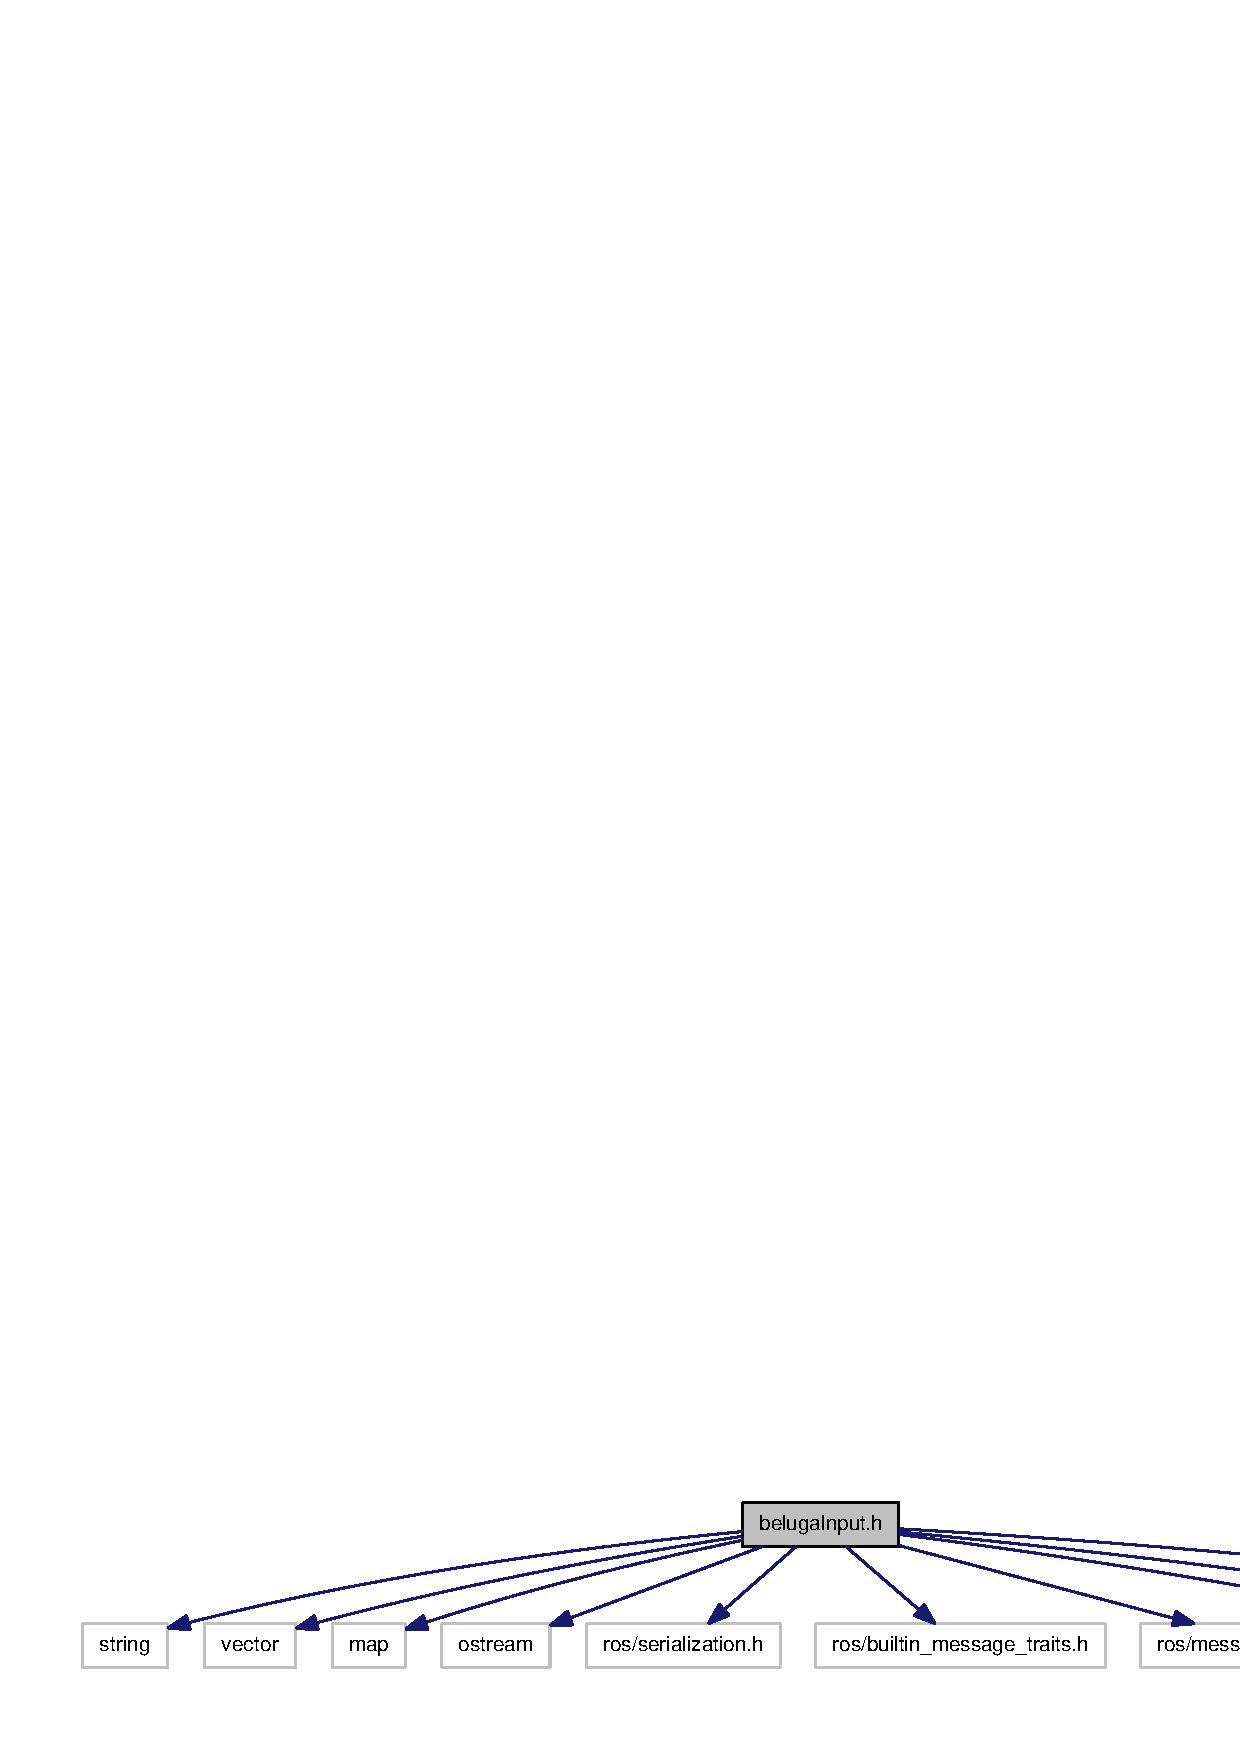
\includegraphics[width=350pt]{belugaInput_8h__incl}
\end{center}
\end{figure}
\subsection*{\-Classes}
\begin{DoxyCompactItemize}
\item 
struct {\bf dcsl\-\_\-messages\-::beluga\-Input\-\_\-$<$ Container\-Allocator $>$}
\item 
struct {\bf ros\-::message\-\_\-traits\-::\-Data\-Type$<$ \-::dcsl\-\_\-messages\-::beluga\-Input\-\_\-$<$ Container\-Allocator $>$ $>$}
\item 
struct {\bf ros\-::message\-\_\-traits\-::\-Definition$<$ \-::dcsl\-\_\-messages\-::beluga\-Input\-\_\-$<$ Container\-Allocator $>$ $>$}
\item 
struct {\bf ros\-::message\-\_\-traits\-::\-Is\-Fixed\-Size$<$ \-::dcsl\-\_\-messages\-::beluga\-Input\-\_\-$<$ Container\-Allocator $>$ $>$}
\item 
struct {\bf ros\-::message\-\_\-traits\-::\-Is\-Message$<$ \-::dcsl\-\_\-messages\-::beluga\-Input\-\_\-$<$ Container\-Allocator $>$ $>$}
\item 
struct {\bf ros\-::message\-\_\-traits\-::\-Is\-Message$<$ \-::dcsl\-\_\-messages\-::beluga\-Input\-\_\-$<$ Container\-Allocator $>$const  $>$}
\item 
struct {\bf ros\-::message\-\_\-traits\-::\-M\-D5\-Sum$<$ \-::dcsl\-\_\-messages\-::beluga\-Input\-\_\-$<$ Container\-Allocator $>$ $>$}
\item 
struct {\bf ros\-::message\-\_\-operations\-::\-Printer$<$ \-::dcsl\-\_\-messages\-::beluga\-Input\-\_\-$<$ Container\-Allocator $>$ $>$}
\item 
struct {\bf ros\-::serialization\-::\-Serializer$<$ \-::dcsl\-\_\-messages\-::beluga\-Input\-\_\-$<$ Container\-Allocator $>$ $>$}
\end{DoxyCompactItemize}
\subsection*{\-Namespaces}
\begin{DoxyCompactItemize}
\item 
namespace {\bf dcsl\-\_\-messages}
\item 
namespace {\bf ros}
\item 
namespace {\bf ros\-::message\-\_\-operations}
\item 
namespace {\bf ros\-::message\-\_\-traits}
\item 
namespace {\bf ros\-::serialization}
\end{DoxyCompactItemize}
\subsection*{\-Typedefs}
\begin{DoxyCompactItemize}
\item 
typedef \*
\-::{\bf dcsl\-\_\-messages\-::beluga\-Input\-\_\-}\*
$<$ std\-::allocator$<$ void $>$ $>$ {\bf dcsl\-\_\-messages\-::beluga\-Input}
\item 
typedef boost\-::shared\-\_\-ptr\*
$<$ \-::{\bf dcsl\-\_\-messages\-::beluga\-Input} \*
const  $>$ {\bf dcsl\-\_\-messages\-::beluga\-Input\-Const\-Ptr}
\item 
typedef boost\-::shared\-\_\-ptr\*
$<$ \-::{\bf dcsl\-\_\-messages\-::beluga\-Input} $>$ {\bf dcsl\-\_\-messages\-::beluga\-Input\-Ptr}
\end{DoxyCompactItemize}
\subsection*{\-Functions}
\begin{DoxyCompactItemize}
\item 
{\footnotesize template$<$typename Container\-Allocator $>$ }\\std\-::ostream \& {\bf dcsl\-\_\-messages\-::operator$<$$<$} (std\-::ostream \&s, const \-::{\bf dcsl\-\_\-messages\-::beluga\-Input\-\_\-}$<$ \-Container\-Allocator $>$ \&v)
\end{DoxyCompactItemize}

\section{mainpage.\-dox \-File \-Reference}
\label{mainpage_8dox}\index{mainpage.\-dox@{mainpage.\-dox}}

\section{\-Twist\-Array.\-h \-File \-Reference}
\label{TwistArray_8h}\index{\-Twist\-Array.\-h@{\-Twist\-Array.\-h}}
{\ttfamily \#include $<$string$>$}\*
{\ttfamily \#include $<$vector$>$}\*
{\ttfamily \#include $<$map$>$}\*
{\ttfamily \#include $<$ostream$>$}\*
{\ttfamily \#include \char`\"{}ros/serialization.\-h\char`\"{}}\*
{\ttfamily \#include \char`\"{}ros/builtin\-\_\-message\-\_\-traits.\-h\char`\"{}}\*
{\ttfamily \#include \char`\"{}ros/message\-\_\-operations.\-h\char`\"{}}\*
{\ttfamily \#include \char`\"{}ros/time.\-h\char`\"{}}\*
{\ttfamily \#include \char`\"{}ros/macros.\-h\char`\"{}}\*
{\ttfamily \#include \char`\"{}ros/assert.\-h\char`\"{}}\*
{\ttfamily \#include \char`\"{}std\-\_\-msgs/\-Header.\-h\char`\"{}}\*
{\ttfamily \#include \char`\"{}geometry\-\_\-msgs/\-Twist.\-h\char`\"{}}\*
\-Include dependency graph for \-Twist\-Array.\-h\-:
\nopagebreak
\begin{figure}[H]
\begin{center}
\leavevmode
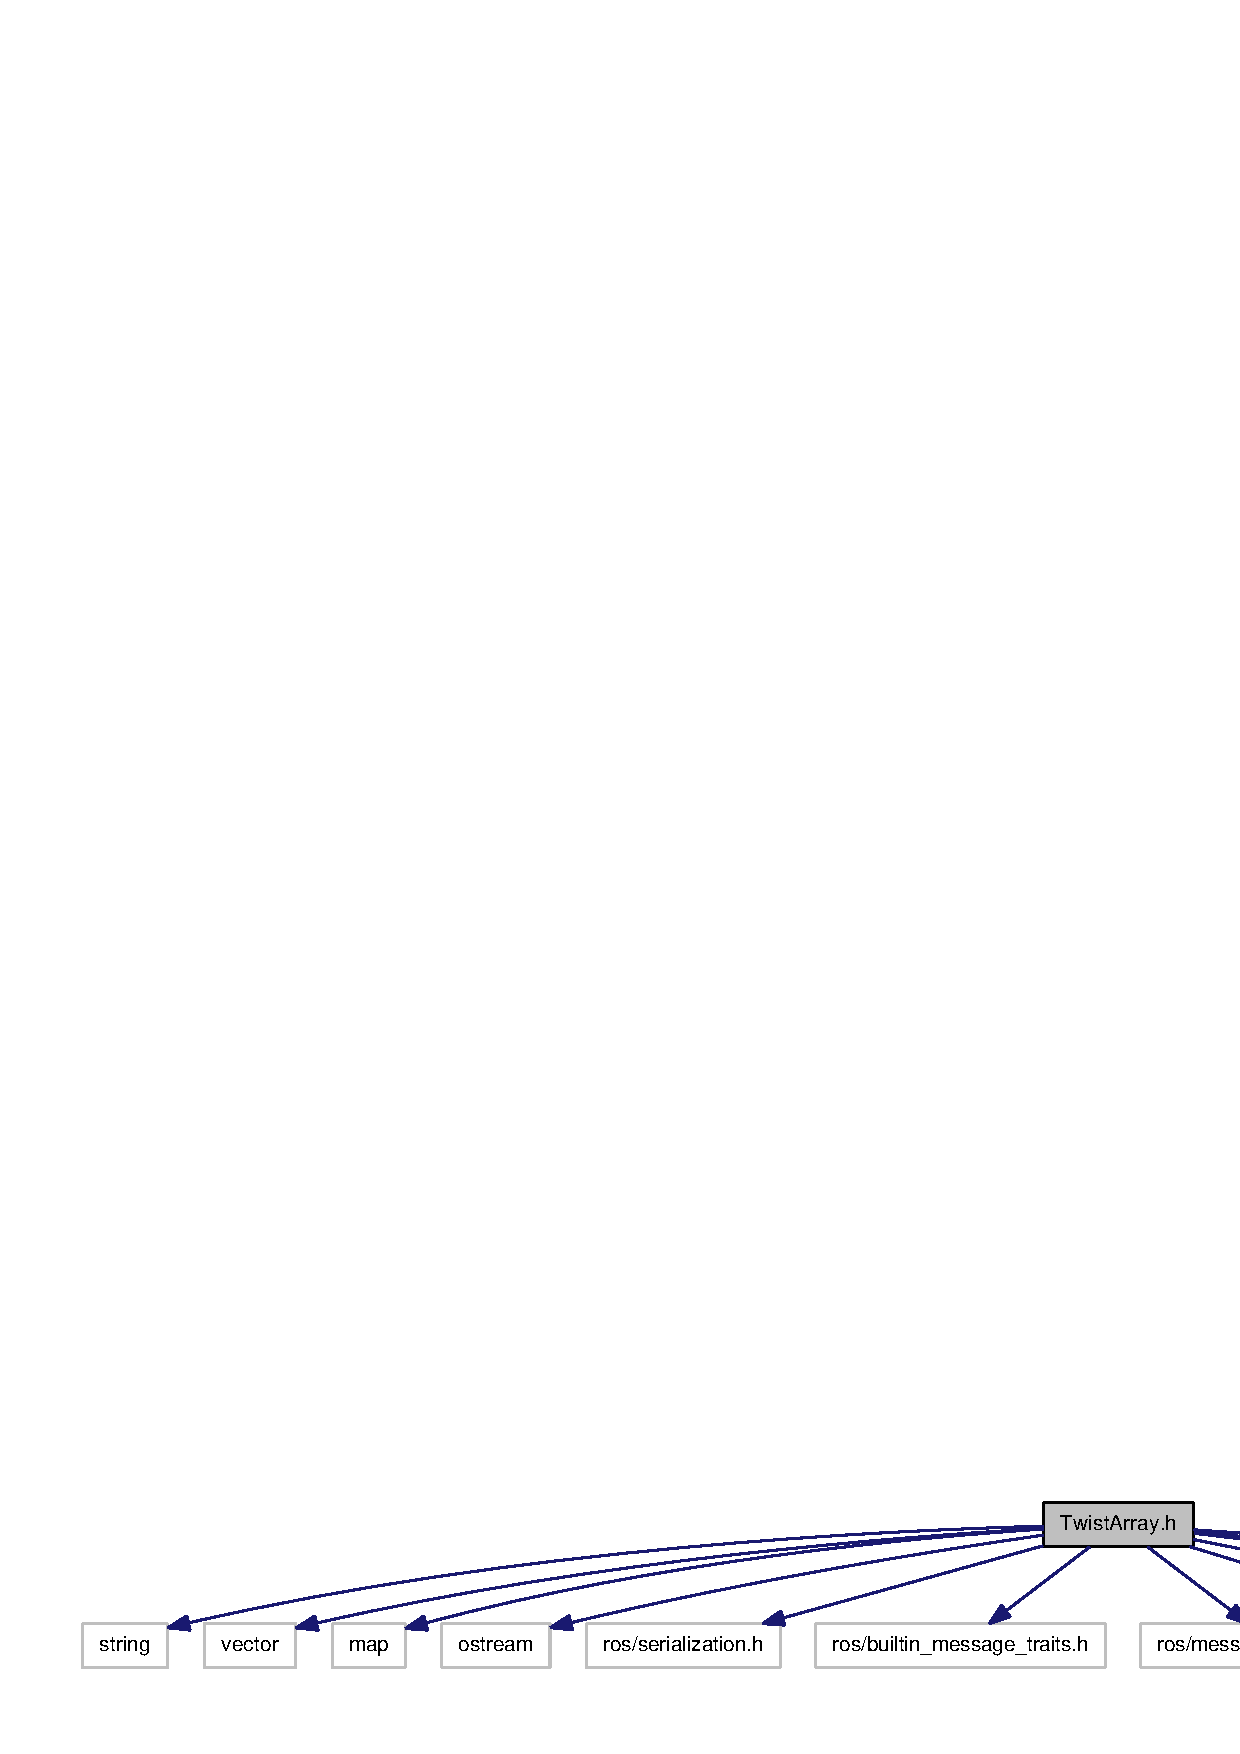
\includegraphics[width=350pt]{TwistArray_8h__incl}
\end{center}
\end{figure}
\subsection*{\-Classes}
\begin{DoxyCompactItemize}
\item 
struct {\bf ros\-::message\-\_\-traits\-::\-Data\-Type$<$ \-::dcsl\-\_\-messages\-::\-Twist\-Array\-\_\-$<$ Container\-Allocator $>$ $>$}
\item 
struct {\bf ros\-::message\-\_\-traits\-::\-Definition$<$ \-::dcsl\-\_\-messages\-::\-Twist\-Array\-\_\-$<$ Container\-Allocator $>$ $>$}
\item 
struct {\bf ros\-::message\-\_\-traits\-::\-Has\-Header$<$ \-::dcsl\-\_\-messages\-::\-Twist\-Array\-\_\-$<$ Container\-Allocator $>$ $>$}
\item 
struct {\bf ros\-::message\-\_\-traits\-::\-Has\-Header$<$ const \-::dcsl\-\_\-messages\-::\-Twist\-Array\-\_\-$<$ Container\-Allocator $>$ $>$}
\item 
struct {\bf ros\-::message\-\_\-traits\-::\-Is\-Message$<$ \-::dcsl\-\_\-messages\-::\-Twist\-Array\-\_\-$<$ Container\-Allocator $>$ $>$}
\item 
struct {\bf ros\-::message\-\_\-traits\-::\-Is\-Message$<$ \-::dcsl\-\_\-messages\-::\-Twist\-Array\-\_\-$<$ Container\-Allocator $>$const  $>$}
\item 
struct {\bf ros\-::message\-\_\-traits\-::\-M\-D5\-Sum$<$ \-::dcsl\-\_\-messages\-::\-Twist\-Array\-\_\-$<$ Container\-Allocator $>$ $>$}
\item 
struct {\bf ros\-::message\-\_\-operations\-::\-Printer$<$ \-::dcsl\-\_\-messages\-::\-Twist\-Array\-\_\-$<$ Container\-Allocator $>$ $>$}
\item 
struct {\bf ros\-::serialization\-::\-Serializer$<$ \-::dcsl\-\_\-messages\-::\-Twist\-Array\-\_\-$<$ Container\-Allocator $>$ $>$}
\item 
struct {\bf dcsl\-\_\-messages\-::\-Twist\-Array\-\_\-$<$ Container\-Allocator $>$}
\end{DoxyCompactItemize}
\subsection*{\-Namespaces}
\begin{DoxyCompactItemize}
\item 
namespace {\bf dcsl\-\_\-messages}
\item 
namespace {\bf ros}
\item 
namespace {\bf ros\-::message\-\_\-operations}
\item 
namespace {\bf ros\-::message\-\_\-traits}
\item 
namespace {\bf ros\-::serialization}
\end{DoxyCompactItemize}
\subsection*{\-Typedefs}
\begin{DoxyCompactItemize}
\item 
typedef \*
\-::{\bf dcsl\-\_\-messages\-::\-Twist\-Array\-\_\-}\*
$<$ std\-::allocator$<$ void $>$ $>$ {\bf dcsl\-\_\-messages\-::\-Twist\-Array}
\item 
typedef boost\-::shared\-\_\-ptr\*
$<$ \-::{\bf dcsl\-\_\-messages\-::\-Twist\-Array} \*
const  $>$ {\bf dcsl\-\_\-messages\-::\-Twist\-Array\-Const\-Ptr}
\item 
typedef boost\-::shared\-\_\-ptr\*
$<$ \-::{\bf dcsl\-\_\-messages\-::\-Twist\-Array} $>$ {\bf dcsl\-\_\-messages\-::\-Twist\-Array\-Ptr}
\end{DoxyCompactItemize}
\subsection*{\-Functions}
\begin{DoxyCompactItemize}
\item 
{\footnotesize template$<$typename Container\-Allocator $>$ }\\std\-::ostream \& {\bf dcsl\-\_\-messages\-::operator$<$$<$} (std\-::ostream \&s, const \-::{\bf dcsl\-\_\-messages\-::\-Twist\-Array\-\_\-}$<$ \-Container\-Allocator $>$ \&v)
\end{DoxyCompactItemize}

\printindex
\end{document}
